%% LyX 2.3.6.2 created this file.  For more info, see http://www.lyx.org/.
%% Do not edit unless you really know what you are doing.
\documentclass[english]{revtex4-1}
\usepackage[T1]{fontenc}
\usepackage[latin9]{inputenc}
\usepackage[a4paper]{geometry}
\geometry{verbose,tmargin=2.5cm,bmargin=2.5cm,lmargin=3cm,rmargin=3cm}
\setcounter{secnumdepth}{3}
\usepackage{color}
\usepackage{babel}
\usepackage{float}
\usepackage{amsmath}
\usepackage{amsthm}
\usepackage{amssymb}
\usepackage{graphicx}
\usepackage[unicode=true,
 bookmarks=true,bookmarksnumbered=true,bookmarksopen=false,
 breaklinks=false,pdfborder={0 0 0},pdfborderstyle={},backref=false,colorlinks=true]
 {hyperref}
\hypersetup{
 pdfauthor={Fabrizio Pittorino},
 pdfstartview=XYZ, plainpages=false, pdfpagelabels}

\makeatletter

%%%%%%%%%%%%%%%%%%%%%%%%%%%%%% LyX specific LaTeX commands.
%% A simple dot to overcome graphicx limitations
\newcommand{\lyxdot}{.}


%%%%%%%%%%%%%%%%%%%%%%%%%%%%%% Textclass specific LaTeX commands.
\@ifundefined{lettrine}{\usepackage{lettrine}}{}
\numberwithin{equation}{section}
\numberwithin{figure}{section}
\numberwithin{table}{section}

%%%%%%%%%%%%%%%%%%%%%%%%%%%%%% User specified LaTeX commands.
\DeclareMathOperator\atanh{atanh}
\DeclareMathOperator\sign{sign}
\DeclareMathOperator\erfcx{erfcx}


\usepackage[T1]{fontenc}
\setcounter{secnumdepth}{3}
\usepackage{color}
\usepackage{babel}
\usepackage{mathrsfs}
\usepackage{amsmath}
\usepackage{amssymb}
\usepackage{graphicx}
%\usepackage[unicode=true,pdfusetitle, bookmarks=true,bookmarksnumbered=false,bookmarksopen=false, breaklinks=false,pdfborder={0 0 0},pdfborderstyle={},backref=false,colorlinks=true]{hyperref}
\hypersetup{
 linkcolor=burntgreen,citecolor=red,urlcolor=burntorange}

\makeatletter

%%%%%%%%%%%%%%%%%%%%%%%%%%%%%% User specified LaTeX commands.
\usepackage{color}
\definecolor{burntorange}{rgb}{0.8, 0.33, 0.0}
\definecolor{charcoal}{rgb}{0.21, 0.27, 0.31}
\definecolor{coolblack}{rgb}{0.0, 0.28, 0.49}
\definecolor{burntgreen}{rgb}{0.05, 0.45, 0.27}
\definecolor{burntblue}{rgb}{0.05, 0.27, 0.8}

\setcitestyle{authoryear,round}
\setlength{\bibsep}{2mm}

\makeatother

\bibliography{refs.bib}

\makeatother

\begin{document}
\title{Deep Message Passing}
\begin{abstract}
Around the middle of the XVII century, a young man called Baruch Spinoza
was dealing with a problem tougher than yours: finding the essence
of God Himself.

\tableofcontents{}
\end{abstract}
\maketitle

\section{Introduction}

\section{Learning through message passing}

TODO ENTIRE SECTION.

In this deep inference problem, we assume that a signal with prior
$P^{\text{in}}$ is fed to a deep feedforward networks with $L+1$
layers of weights $\boldsymbol{W}^{\ell}\in\mathbb{R}^{N_{\ell+1}\times N_{\ell}},\ell=0,\dots,L$
and biases $\boldsymbol{b}^{\ell}\in\text{\ensuremath{\mathbb{R}^{N_{\ell+1}}}}$.
The signal is propagated through stochastic neuron layers described
by probability distributions $P^{\ell}$ conditioned on the preactivations,
therefore we have the following Markov chain:

\begin{align}
\boldsymbol{x}^{0} & \sim P^{\text{in}}\\
\boldsymbol{x}^{\ell+1} & \sim P^{\ell+1}\left(\bullet\,|\,\boldsymbol{W}^{\ell}\boldsymbol{x}^{\ell}+\boldsymbol{b}^{\ell}\right)\qquad\ell=0,\dots,L
\end{align}

Only $\boldsymbol{y}=\boldsymbol{x}^{L+1}$ is observed, and the task
is to reconstruct the original signal $\boldsymbol{x}^{0}$. The posterior
distribution $p(\boldsymbol{x}^{0:L})=P(\boldsymbol{x}^{0:L}\,|\,\boldsymbol{x}^{L+1}=\boldsymbol{y})$
reads

\begin{align}
p(\boldsymbol{x}^{0:L}) & \propto\prod_{\ell=0}^{L}\prod_{k=1}^{N_{\ell+1}}\,P_{k}^{\ell+1}\left(x_{k}^{\ell+1}\ \bigg|\ \sum_{i=1}^{N_{\ell}}W_{ki}^{\ell}x_{i}^{\ell}\right)\ \prod_{k=1}^{N_{0}}P_{k}^{\text{in}}(x_{k}^{0}),
\end{align}

Typical channels are given by deterministic elementwise activation
function $f_{\ell}(z)$ (e.g. $f_{\ell}(z)=\sign(x)$ or $f_{\ell}(z)=\text{relu}(z)=\max(0,z)$),
combined with Gaussian additive pre-activation noise with variance
$\sigma^{2}$. In such cases we have

\[
P_{k}^{\ell}(x\,|\,z)=\int D\xi\,\delta\left(x-f_{\ell}(z+\sigma_{k}^{\ell}\,\xi)\right)
\]

We also call $\alpha_{\ell}=N_{\ell+1}/N_{\ell}$ the layer \emph{expansion
ratio.}

\section{Belief Propagation}

\subsection{BP updates}

The AMP equations have been derived from the BP equation in the Appendix.
First we introduce the neuron scalar entropy functions:
\begin{align}
\varphi_{k}^{0}(B,A) & =\log\int\mathrm{d}x\ e^{-\frac{1}{2}A^{2}x^{2}+Bx}\,P_{k}^{\text{in}}(x)\\
\varphi_{k}^{\ell}(B,A,\omega,V) & =\log\int\mathrm{d}x\,\mathrm{d}z\ e^{-\frac{1}{2}A^{2}x^{2}+Bx}\,P_{k}^{\ell}\left(x|z\right)e^{-\frac{(\omega-z)^{2}}{2V}}\qquad\ell=1,\dots,L\\
\varphi_{k}^{L+1}(\omega,V,y) & =\log\int\mathrm{d}z\ P_{k}^{L+1}\left(y|z\right)e^{-\frac{(\omega-z)^{2}}{2V}}\\
\psi_{ki}^{\ell}(H,G) & =\log\int\mathrm{d}w\ e^{-\frac{1}{2}G^{2}w^{2}+Hw}\,P_{ki}^{\text{\ensuremath{\ell}}}(w)
\end{align}

For convenience define $\varphi_{i}^{0,t}=\varphi_{i}^{0}\left(B_{i}^{0,t},A_{i}^{0,t}\right)$
and $\varphi_{i}^{\ell,t}=\varphi_{i}^{\ell}\left(B_{i}^{\ell,t},A_{i}^{\ell,t},\omega_{i}^{\ell-1,t},V_{i}^{\ell-1,t}\right)$
and $\varphi_{i}^{L+1,t}=\varphi_{i}^{L+1}\left(\omega_{i}^{L,t},V_{i}^{L,t},y_{i}\right)$. 

Then, we can decompose the BP update rules in a forward and a backward
step.

\paragraph{Forward pass.}

As the initial condition for the iterations, we set to zero the following
quantities: $B_{i}^{\ell,t=0}=0,A_{i}^{\ell,t=0}=0$ and $g_{k}^{\ell,t=0}=0$.
The following iterations hold at time $t\geq1$. In the FORWARD pass,
starting from $\ell=0$ and up to $\ell=L$, we have

\begin{align}
\hat{x}_{ia\to k}^{\ell,t} & =\partial_{B}\varphi_{ia\to k}^{\ell}\left(B_{ia\to k}^{\ell,t-1},A_{ia}^{\ell,t-1},\omega_{ia}^{\ell-1,t},V_{ia}^{\ell-1,t}\right)\\
\Delta_{ia\to k}^{\ell+1,t} & =\partial_{B}^{2}\varphi_{ia\to k}^{\ell+1,t}\\
m_{ki\to a}^{\ell,t} & =\partial_{H}\psi_{ki}^{\ell}(H_{ki\to a}^{t-1},G_{ki}^{t-1})\\
\sigma_{ki\to a}^{\ell,t} & =\partial_{H}^{2}\psi_{ki}^{\ell}(H_{ki\to a}^{t-1},G_{ki}^{t-1})\\
V_{ka}^{\ell,t} & =\sum_{i}\left(\left(m_{ki\to a}^{\ell,t}\right)^{2}\Delta_{ia\to k}^{\ell,t}+\Sigma_{ki\to a}^{\ell,t}(\hat{x}_{ia\to k}^{\ell,t})^{2}+\sigma_{ki\to a}^{\ell,t}\Delta_{ia\to k}^{\ell,t}\right)\label{eq:upd-V-2}\\
\omega_{ka\to i}^{\ell,t} & =\sum_{i'\neq i}m_{ki\to a}^{\ell,t}\hat{x}_{ia\to k}^{\ell,t}\label{eq:upd-w-2}
\end{align}

Here $V^{\ell}$ and $\omega^{\ell}$ are computed as a function of
the previous layer values $V^{\ell-1}$ and $\omega^{\ell-1}$. 

\paragraph{Backward pass.}

In the BACKWARD sweep, starting from $\ell=L$ and down to $\ell=0$,
we have 

\begin{align}
g_{ka\to i}^{\ell,t} & =\partial_{\omega}\varphi_{ka\to i}^{\ell+1}\left(B_{ka}^{\ell+1,t},A_{ka}^{\ell+1,t},\omega_{ka\to i}^{\ell,t},V_{ka}^{\ell,t}\right)\label{eq:upd-g-2}\\
\Gamma_{ka\to i}^{\ell,t} & =-\partial_{\omega}^{2}\varphi_{ka\to i}^{\ell+1,t}\label{eq:upd-dwg-2}\\
A_{ia}^{\ell,t} & =\sum_{k}\left((m_{ki\to a}^{\ell,t})^{2}+\sigma_{ki\to a}^{\ell,t}\right)\Gamma_{ka\to i}^{\ell,t}-\sigma_{ki\to a}^{\ell,t}\left(g_{ka\to i}^{\ell,t}\right)^{2}\label{eq:upd-A-2}\\
B_{ia\to k}^{\ell,t} & =\sum_{k'\neq k}m_{k'i\to a}^{\ell}g_{k'a\to i}^{\ell,t}\label{eq:upd-B-2}\\
G_{ki}^{\ell,t} & =\sum_{a}\left((\hat{x}_{ia\to k}^{\ell,t})^{2}+\Delta_{ia\to k}\right)\Gamma_{ka\to i}^{\ell,t}-\Delta_{ia\to k}\left(g_{ka\to i}^{\ell,t}\right)^{2}\\
H_{ki\to a} & =\sum_{a'\neq a}\hat{x}_{ia'\to k}^{\ell,t}g_{ka'\to i}^{\ell,t}
\end{align}

Notice that $A^{\ell}$ and $B^{\ell}$ are computed as as a function
of the $A^{\ell+1},B^{\ell+1}$ of the layer above, with the initial
condition given by the output $\boldsymbol{x}^{L+1}=\boldsymbol{y}$
on the top layer.

\subsection{Approximate Message Passing}

\paragraph{Forward pass.}

As the initial condition for the iterations, we set to zero the following
quantities: $B_{i}^{\ell,t=0}=0,A_{i}^{\ell,t=0}=0$ and $g_{k}^{\ell,t=0}=0$.
The following iterations hold at time $t\geq1$. In the FORWARD pass,
starting from $\ell=0$ and up to $\ell=L$, we have

\begin{align}
\hat{x}_{ia}^{\ell,t} & =\partial_{B}\varphi_{ia}^{\ell,t^{-}}\label{eq:upd-h-2-1}\\
\Delta_{ia}^{\ell,t} & =\partial_{B}^{2}\varphi_{ia}^{\ell,t^{-}}\label{eq:upd-sigma-2-1}\\
m_{ki}^{\ell,t} & =\partial_{H}\psi_{ki}^{\ell,t^{-}}\\
\sigma_{ki}^{\ell,t} & =\partial_{H}^{2}\psi_{ki}^{\ell,t^{-}}\\
V_{ka}^{\ell,t} & =\sum_{i}\left(\left(m_{ki}^{\ell,t}\right)^{2}\Delta_{ia}^{\ell,t}+\sigma_{ki}^{\ell,t}(\hat{x}_{ia}^{\ell,t})^{2}+\sigma_{ki}^{\ell,t}\Delta_{ia}^{\ell,t}\right)\label{eq:upd-V-2-1}\\
\omega_{ka}^{\ell,t} & =\sum_{i}m_{ki}^{\ell,t}\hat{x}_{ia}^{\ell,t}+TODO:onsagsize(x)er\label{eq:upd-w-2-1}
\end{align}

Here $V^{\ell}$ and $\omega^{\ell}$ are computed as a function of
the previous layer values $V^{\ell-1}$ and $\omega^{\ell-1}$. 

\paragraph{Backward pass.}

In the BACKWARD sweep, starting from $\ell=L$ and up to $\ell=0$,
we have 

\begin{align}
g_{ka}^{\ell,t} & =\partial_{\omega}\varphi_{ka}^{\ell+1,t}\label{eq:upd-g-2-1}\\
\Gamma_{ka}^{\ell,t} & =-\partial_{\omega}^{2}\varphi_{ka}^{\ell+1,t}\label{eq:upd-dwg-2-1}\\
A_{ia}^{\ell,t} & =\sum_{k}\left((m_{ki}^{\ell,t})^{2}+\sigma_{ki}^{\ell,t}\right)\Gamma_{ka}^{\ell,t}-\sigma_{ki}^{\ell,t}\left(g_{ka}^{\ell,t}\right)^{2}\label{eq:upd-A-2-1}\\
B_{ia}^{\ell,t} & =\sum_{k}m_{ki}^{\ell}g_{ka}^{\ell,t}+TODO:onsager\label{eq:upd-B-2-1}\\
G_{ki}^{\ell,t} & =\sum_{a}\left((\hat{x}_{ia}^{\ell,t})^{2}+\Delta_{ia}\right)\Gamma_{ka}^{\ell,t}-\Delta_{ia}\left(g_{ka}^{\ell,t}\right)^{2}\\
H_{ki} & =\sum_{a}\hat{x}_{ia}^{\ell,t}g_{ka}^{\ell,t}+TODO:onsager
\end{align}

Notice that $A^{\ell}$ and $B^{\ell}$ are computed as as a function
of the $A^{\ell+1},B^{\ell+1}$ of the layer above, with the initial
condition given by the output $\boldsymbol{x}^{L+1}=\boldsymbol{y}$
on the top layer.

\section{ArgMax layer}

In order to perform multi-class classification, we have perform an
argmax operation. Call $z_{k}$, for $k=1,\dots,K$, the Gaussian
random variables output of the last layer of the network in correspondence
of some input $\boldsymbol{x}$. Assuming the correct label is class
$k$, the effective partition function corresponding to the output
constraint reads

\begin{align}
Z_{k^{*}} & =\int\prod_{k}dz_{k}\,\mathcal{N}(z_{k};\omega_{k},V_{k})\ \prod_{k\neq k^{*}}\theta(z_{k^{*}}-z_{k})\\
 & =\int dz_{k^{*}}\,\mathcal{N}(z_{k^{*}};\omega_{k^{*}},V_{k^{*}})\ \prod_{k\neq k^{*}}H\left(-\frac{z_{k^{*}}-\omega_{k}}{\sqrt{V_{k}}}\right)
\end{align}

This last integral is intractable, therefore we have to resort to
approximations.

\subsection{Approach 1: Jensen Inequality}

Using the Jensen inequality we obtain

\begin{align}
\phi_{k^{*}}= & \log Z_{k^{*}}=\log\mathbb{E}_{z\sim\mathcal{N}(\omega_{k^{*}},V_{k^{*}})}\prod_{k\neq k^{*}}H\left(-\frac{z-\omega_{k}}{\sqrt{V_{k}}}\right)\\
 & \geq\sum_{k\neq k^{*}}\mathbb{E}_{z\sim\mathcal{N}(\omega_{k^{*}},V_{k^{*}})}\log H\left(-\frac{z-\omega_{k}}{\sqrt{V_{k}}}\right)
\end{align}

Reparameterizing the expections we have 

\begin{equation}
\tilde{\phi}_{k^{*}}=\sum_{k\neq k^{*}}\mathbb{E}_{\epsilon\sim\mathcal{N}(0,1)}\log H\left(-\frac{\omega_{k^{*}}+\epsilon\sqrt{V_{k^{*}}}-\omega_{k}}{\sqrt{V_{k}}}\right)\label{eq:argmax1}
\end{equation}

The derivative $\partial_{\omega_{k}}\tilde{\phi}_{k^{*}}$ and $\partial_{\omega_{k}}^{2}\tilde{\phi}_{k^{*}}$
that we need can then be estimated by sampling (once?) $\epsilon$.

\begin{equation}
\partial_{\omega_{k}}\tilde{\phi}_{k^{*}}=\begin{cases}
-\frac{1}{\sqrt{V_{k}}}\mathbb{E}_{\epsilon\sim\mathcal{N}(0,1)}\,GH\left(-\frac{\omega_{k^{*}}+\epsilon\sqrt{V_{k^{*}}}-\omega_{k}}{\sqrt{V_{k}}}\right) & k\neq k^{*}\\
\sum_{k'\neq k^{*}}\frac{1}{\sqrt{V_{k'}}}\mathbb{E}_{\epsilon\sim\mathcal{N}(0,1)}\,GH\left(-\frac{\omega_{k^{*}}+\epsilon\sqrt{V_{k^{*}}}-\omega_{k'}}{\sqrt{V_{k'}}}\right) & k=k^{*}
\end{cases}
\end{equation}


\subsection{Approach 2: Jensen again}

A further simplification is obtained by applying Jensen inequality
again to (\ref{eq:argmax1}) but in the opposite direction. We have
the new effective free energy

\begin{align}
\tilde{\phi}_{k^{*}} & =\sum_{k\neq k^{*}}\log\mathbb{E}_{\epsilon\sim\mathcal{N}(0,1)}H\left(-\frac{\omega_{k^{*}}+\epsilon\sqrt{V_{k^{*}}}-\omega_{k}}{\sqrt{V_{k}}}\right)\\
 & =\sum_{k\neq k^{*}}\log H\left(-\frac{\omega_{k^{*}}-\omega_{k}}{\sqrt{V_{k}+V_{k^{*}}}}\right)
\end{align}

This gives, for $k\neq k^{*}$

\begin{equation}
\partial_{\omega_{k}}\tilde{\phi}_{k^{*}}=\begin{cases}
-\frac{1}{\sqrt{V_{k}+V_{k^{*}}}}\,GH\left(-\frac{\omega_{k^{*}}-\omega_{k}}{\sqrt{V_{k}+V_{k^{*}}}}\right) & k\neq k^{*}\\
\sum_{k'\neq k^{*}}\frac{1}{\sqrt{V_{k'}+V_{k^{*}}}}\,GH\left(-\frac{\omega_{k^{*}}-\omega_{k'}}{\sqrt{V_{k'}+V_{k^{*}}}}\right) & k=k^{*}
\end{cases}
\end{equation}

Notice that $\partial_{\omega_{k^{*}}}\tilde{\phi}_{k^{*}}=-\sum_{k\neq k^{*}}\partial_{\omega_{k}}\tilde{\phi}_{k^{*}}$.
In last formulas we used the definition

\begin{equation}
GH(x)=\frac{G(x)}{H(x)}=\frac{\sqrt{2/\pi}}{\erfcx(x/2)}
\end{equation}


\section{Numerical results}

In this section we study multi-layer perceptrons (MLPs) on a binary
classification task on the Fashion-MNIST dataset (divided arbitrarily
in two classes: the even/odd classes in the original dataset respectively
represent the first/second class in the binary classification task).
We perform experiments on the whole dataset and with a MLP with two
hidden layers of size $101$ (apart from the sections in which we
modify the architecture or the dataset size, or otherwise stated).

NB: if in the figures the title reports ``MNIST'', it should be
``Fashion-MNIST''. 

$M$ and $P$ are the same parameter (the dataset size).

\subsection{Experiments on Fashion-MNIST}

We compare the BP family with binary-SGD without biases and without
additional parameters for batch normalization. In order to keep the
pre-activations of each hidden layer normalized we rescale them by
$\frac{1}{\sqrt{N_{\text{in}}}}$ where $N_{\text{in}}$ is the size
of the previous hidden layer (or the input size in the case of the
preactivations afferent to the first hidden layer).

\subsubsection{Good parameters: batch-size 1 and batch-size 128}

We report that it is possible to find values of the hyper-parameters
such that the BP family has final train/test error comparable with
SGD. In our experiments this holds for generic dataset sizes and batch-sizes,
and for generic MLPs (generic depth / hidden layer size).

In summary, up to now the best hyper-parameters (apart from $P$,
batch-size and $\rho$ that has to be tuned similarly to the learning
rate for SGD) are:
\begin{itemize}
\item $\psi=0.8$
\item $\epsilon init=1$
\item $maxiters=1$ ($r=0$)
\end{itemize}
\begin{center}
\begin{figure}[H]
\begin{centering}
\includegraphics[scale=0.7]{\string"figures/deepMP_bs1_K[784, 501, 501, 501, 1]_rho1.0e-6__0.8_P60000.0_maxiters_1_r0.0_init_1.0_\string".png}
\par\end{centering}
\begin{centering}
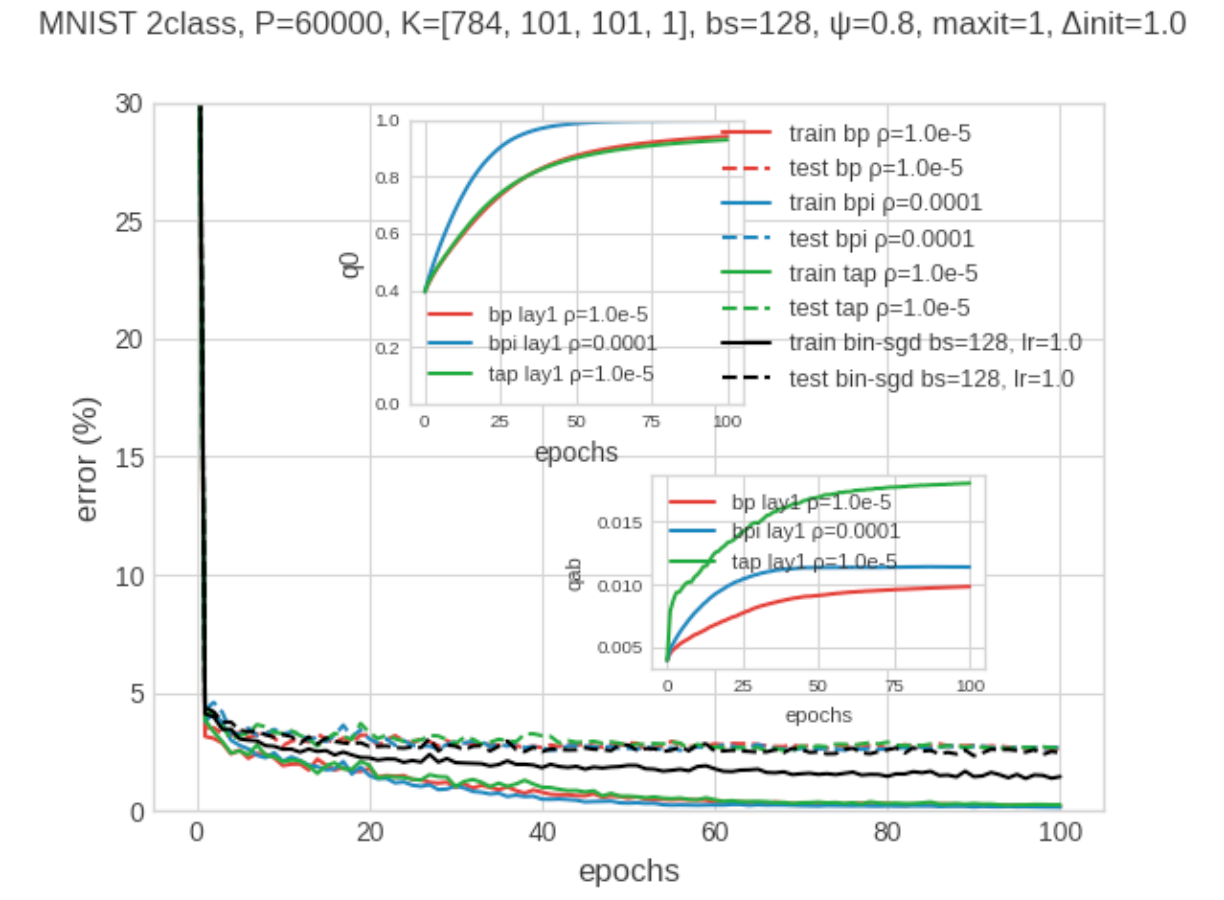
\includegraphics[scale=0.25]{figures/pasted/pasted25}
\par\end{centering}
\caption{Left panel: MLP with 3 hidden layers with 501 hidden units each, batch-size=1
on the Fashion-MNIST dataset. Right panel: MLP with 2 hidden layers
with 101 hidden units each, batch-size=128 on the Fashion-MNIST dataset.
Here we have selected some \textquotedblleft good\textquotedblright{}
values of the parameters. \textbf{NB: in all figures the upper inset
is the self-overlap of the first layer, while the lower inset is the
mean overlap of the couples of sub-perceptrons in the first layer.}}
\end{figure}
\par\end{center}

\subsubsection{Varying batch-size: computational performance}

Here we vary only the batchsize (per completezza farlo per un buon
set degli altri iperparametri), in order to compare the performance
(time) of BP with binary-SGD (both on GPUs).

The command to reproduce the experiments in this section is:

\textcolor{blue}{run\_experiment(9; M=Int(6e4), batchsize=batchsize,
usecuda=true, gpu\_id=0, $\rho$=1+1e-5, $\psi$=0.5, lay=lay, epochs=100)}

with batchsize=\{1,16,128,1024\} and lay=\{:bp, :bpi, :tap\}.
\begin{center}
\begin{figure}[H]
\begin{centering}
\includegraphics[scale=0.5]{\string"figures/deepMP_bs1_K[784, 101, 101, 1]_comparison\string".png}\includegraphics[scale=0.5]{\string"figures/deepMP_bs16_K[784, 101, 101, 1]_comparison\string".png}
\par\end{centering}
\begin{centering}
\includegraphics[scale=0.5]{\string"figures/deepMP_bs128_K[784, 101, 101, 1]_comparison\string".png}\includegraphics[scale=0.5]{\string"figures/deepMP_bs1024_K[784, 101, 101, 1]_comparison\string".png}
\par\end{centering}
\caption{Comparison of BP, TAP, BPI, SGD varying the batchsize (upper left:
bs=1; upper right: bs=16, lower left: bs=128; lower right=1024). The
parameter $\rho-1$ is fixed in all experiments to $10^{-5}$.}

\end{figure}
\par\end{center}

\begin{center}
\begin{figure}[H]
\begin{centering}
\includegraphics[scale=0.75]{\string"figures/deepMP_times_K[784, 101, 101, 1]\string".png}
\par\end{centering}
\caption{Algorithms time scaling with the batchsize. The reported time refers
to one epoch for each algorithm.}
\end{figure}
\par\end{center}

\subsection{Experiments on Fashion-MNIST: parameters}

Here we stick to batchsize 128 and we vary the other hyperparameters.
However, we expect that some of the parameters scale with the batchsize
(in particular we expect $\rho-1\propto\frac{\text{batchsize}}{\text{data set size}}$).

The command to reproduce the experiments is along the lines of:

run\_experiment(9; usecuda=true, gpu\_id=0, epochs=100, lay=\{:bp,
:bpi, :tap, :mf\}, batchsize=128, $\rho$=$\star$, $\psi$=0.8, M=Int(6e4),
maxiters=1, r=0., $\epsilon init=1$, K={[}28{*}28,101,101,1{]})

\subsubsection{Varying $\rho$}

$\rho$s = {[}-1e-1, -1e-5, 0., 1e-7, 1e-6, 1e-5, 1e-4, 1e-3, 1e-2,
1e-1{]} .+ 1. 

For $bs=128$ we choose $\rho-1=10^{-5}$ for bp, bpi, tap and $10^{-4}$
for mf. The command is the same as the one in the first paragraph
of section B except for $\rho$.
\begin{center}
\begin{figure}[H]
\begin{centering}
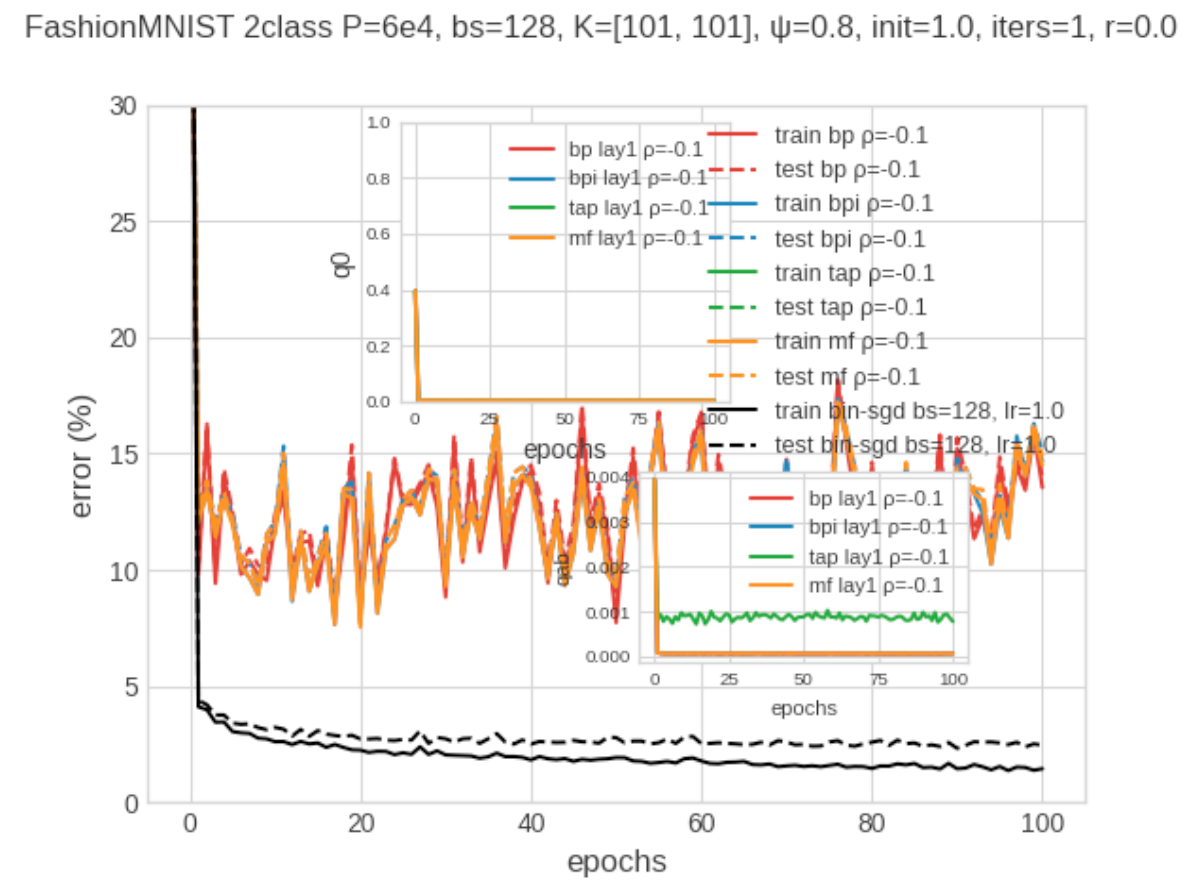
\includegraphics[scale=0.2]{figures/pasted_new/pasted9}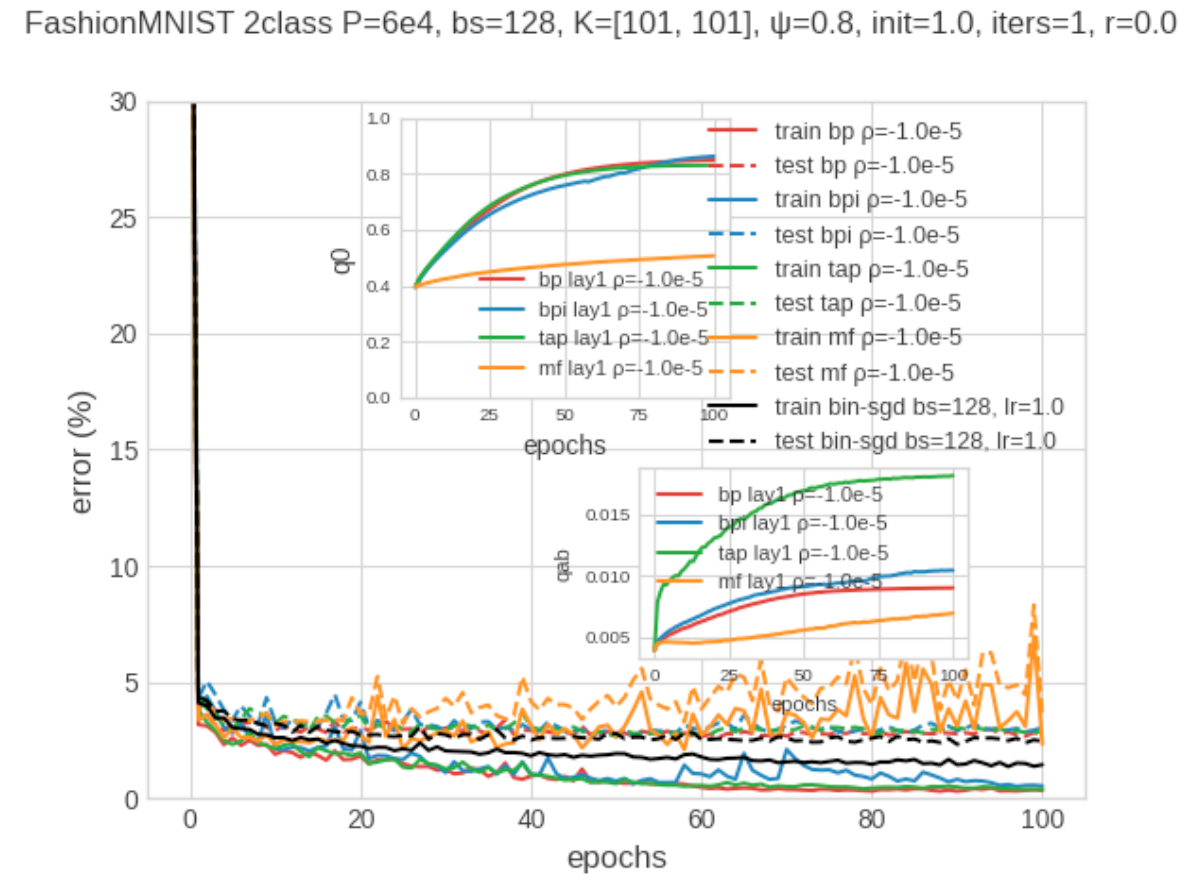
\includegraphics[scale=0.2]{figures/pasted_new/pasted10}
\par\end{centering}
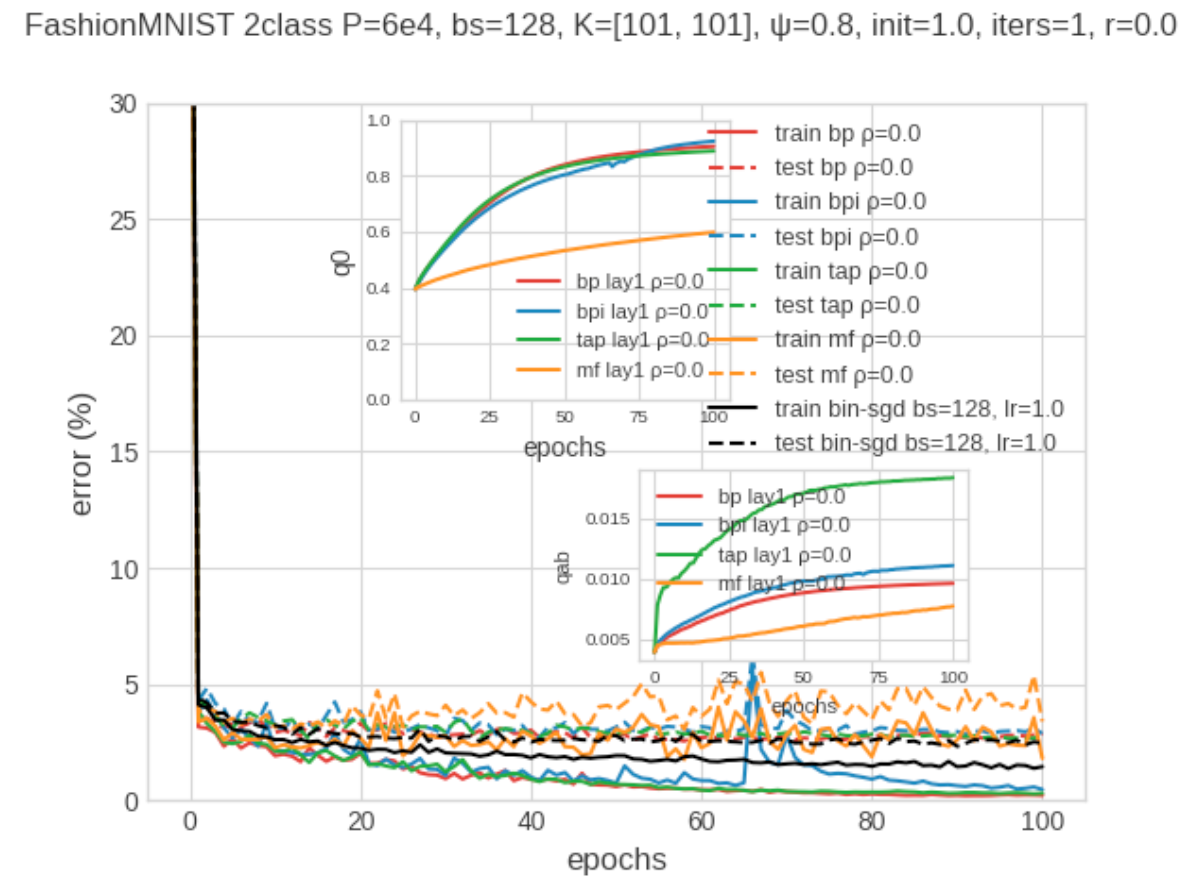
\includegraphics[scale=0.2]{figures/pasted_new/pasted11}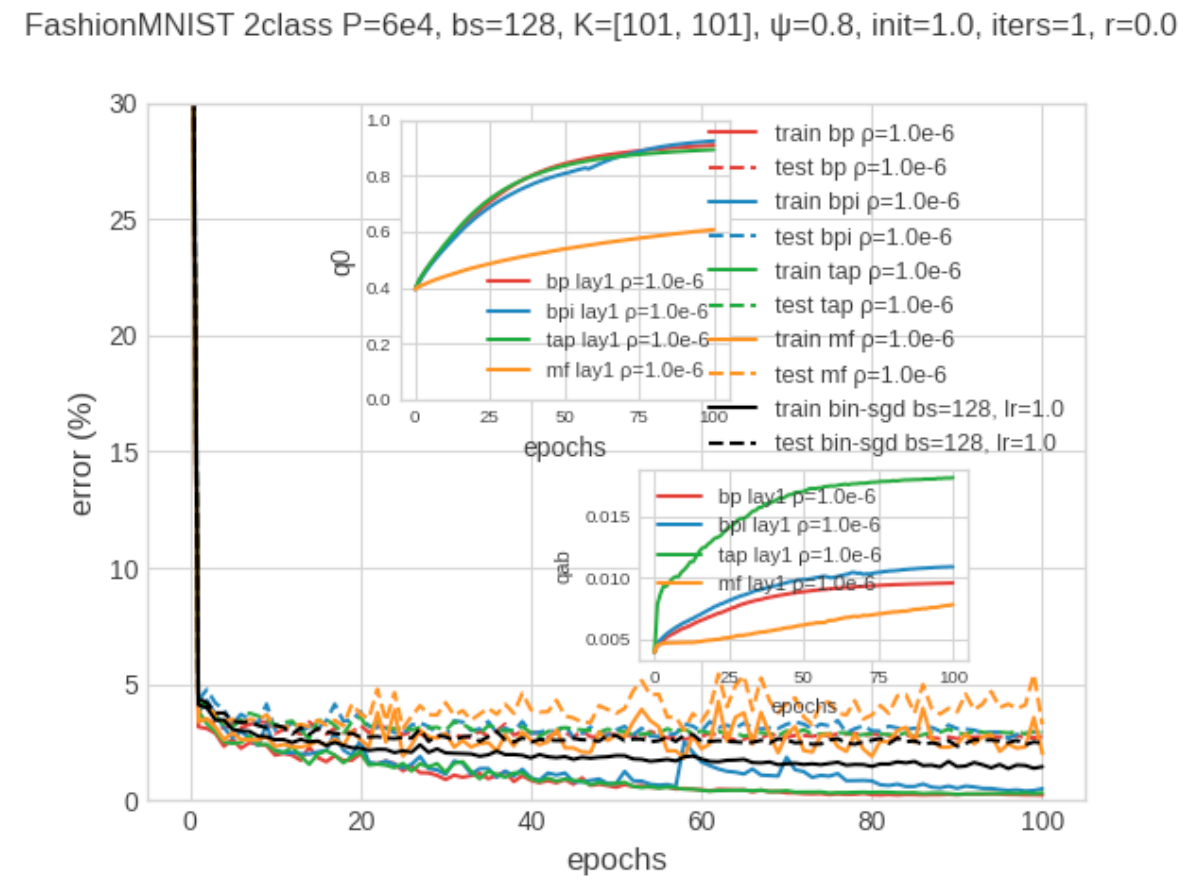
\includegraphics[scale=0.2]{figures/pasted_new/pasted12}

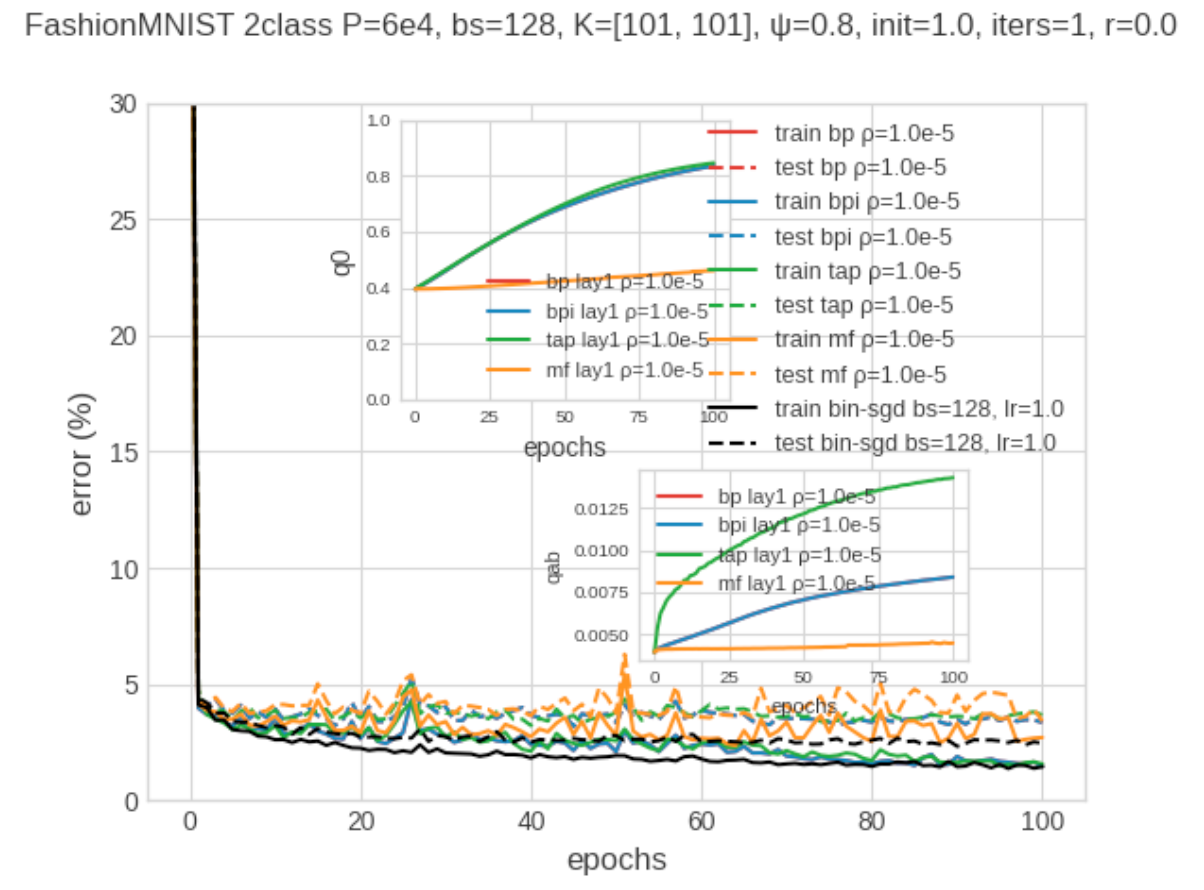
\includegraphics[scale=0.2]{figures/pasted_new/pasted13}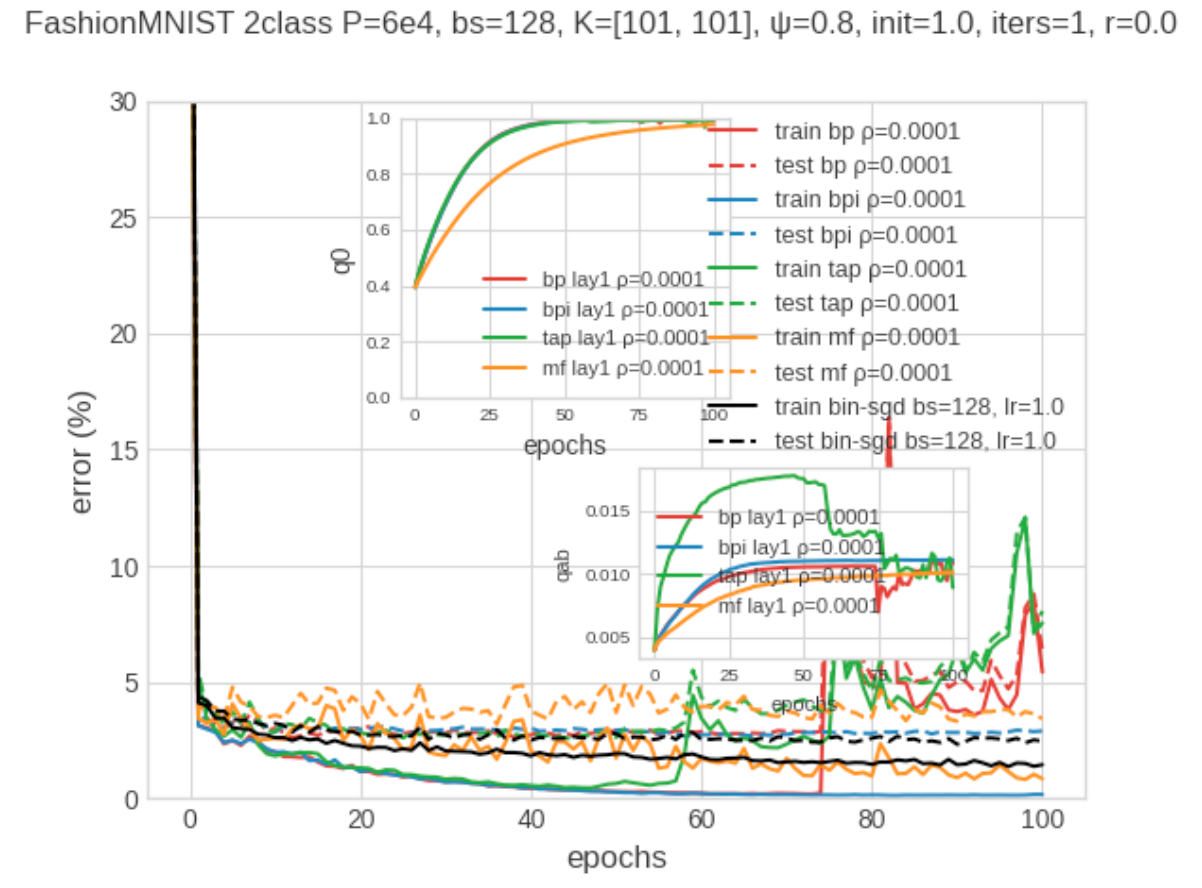
\includegraphics[scale=0.2]{figures/pasted_new/pasted14}

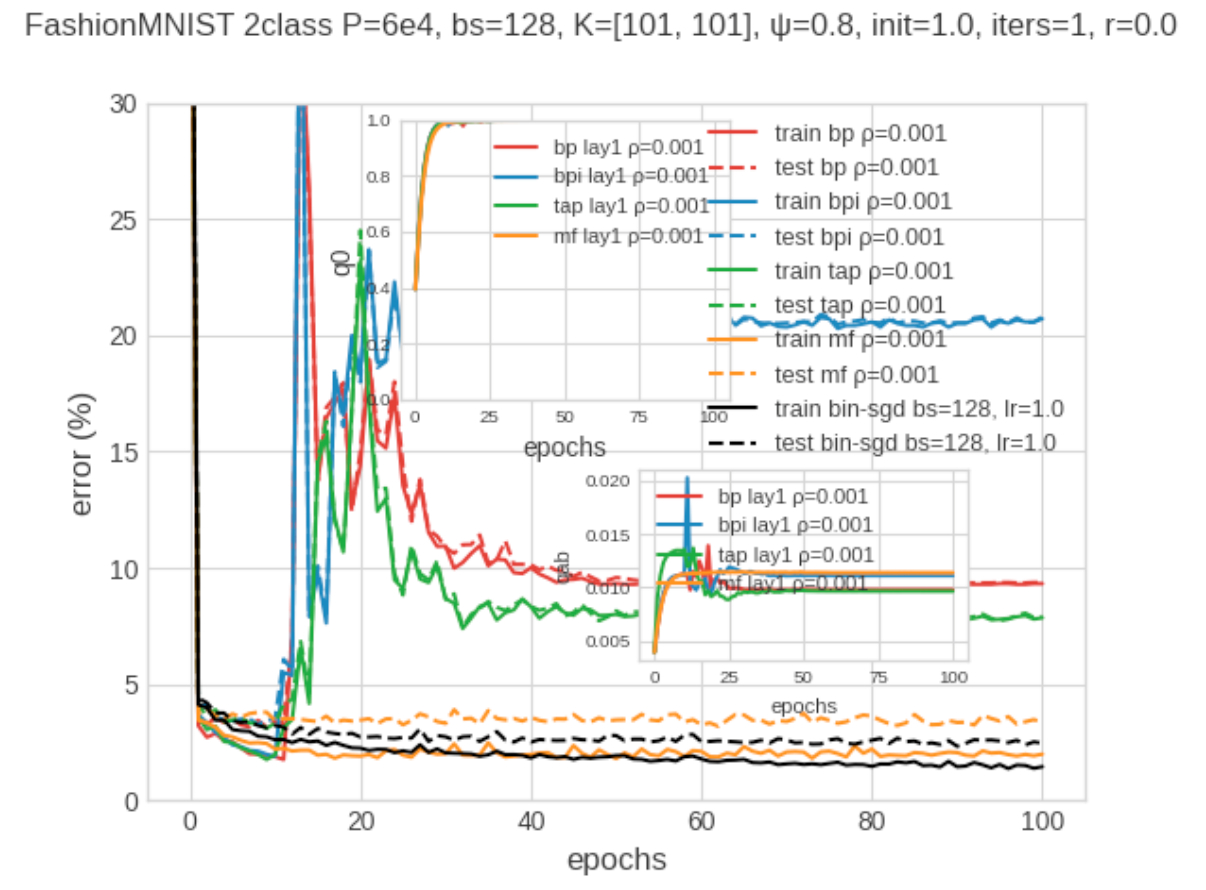
\includegraphics[scale=0.2]{figures/pasted_new/pasted15}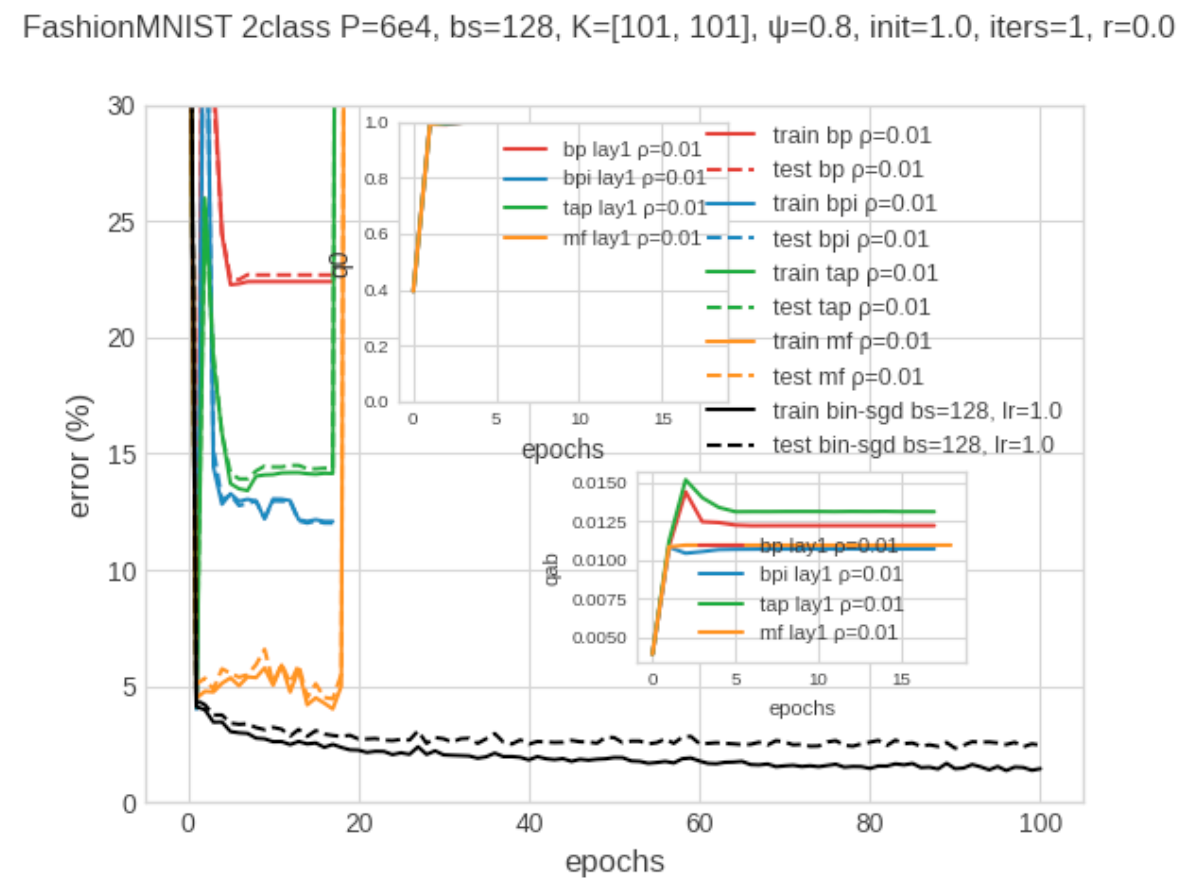
\includegraphics[scale=0.2]{figures/pasted_new/pasted16}

\caption{MLP with 2 hidden layers with 101 hidden units each, batch-size=128
on the Fashion-MNIST dataset. We vary the parameter $\rho$.}
\end{figure}
\par\end{center}

\subsubsection{Varying initial weights}

$\epsilon$inits = {[}0., 0.01, 0.1, 0.5, 1, 1.5, 2, 3{]}
\begin{center}
\begin{figure}[H]
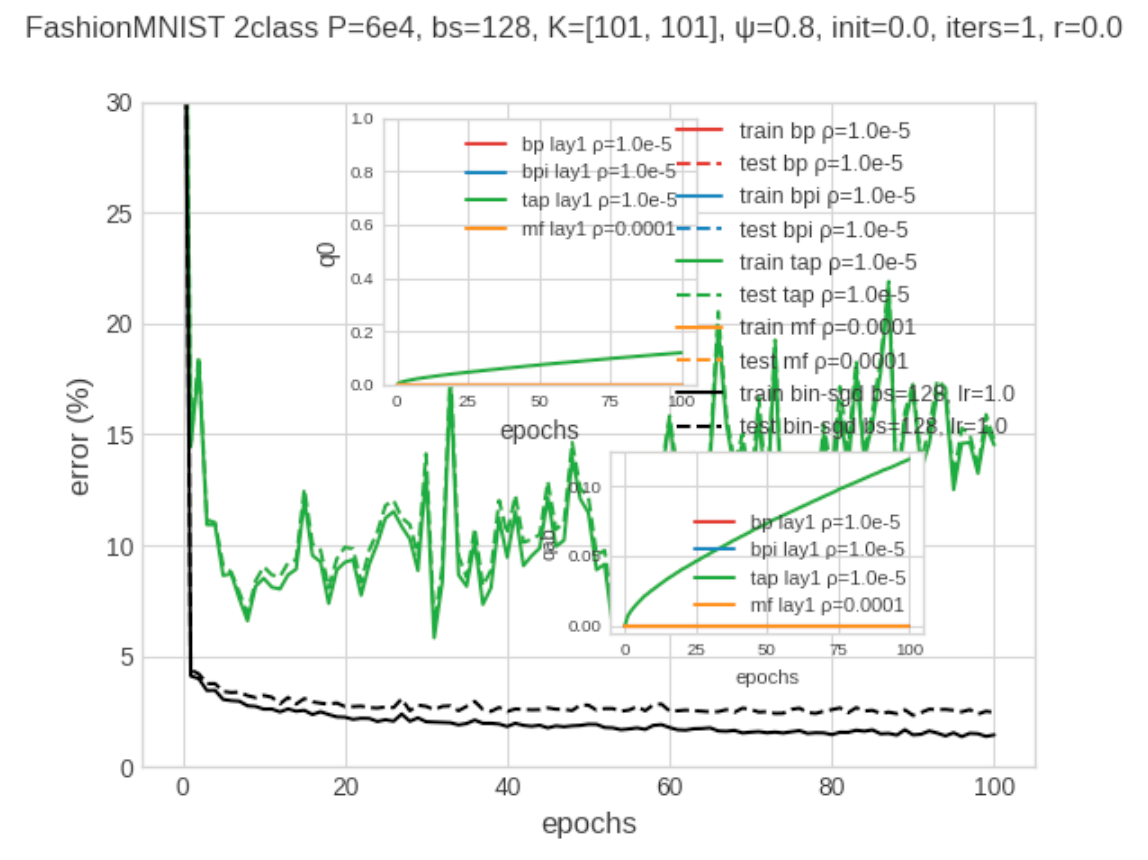
\includegraphics[scale=0.2]{figures/pasted_new/pasted6}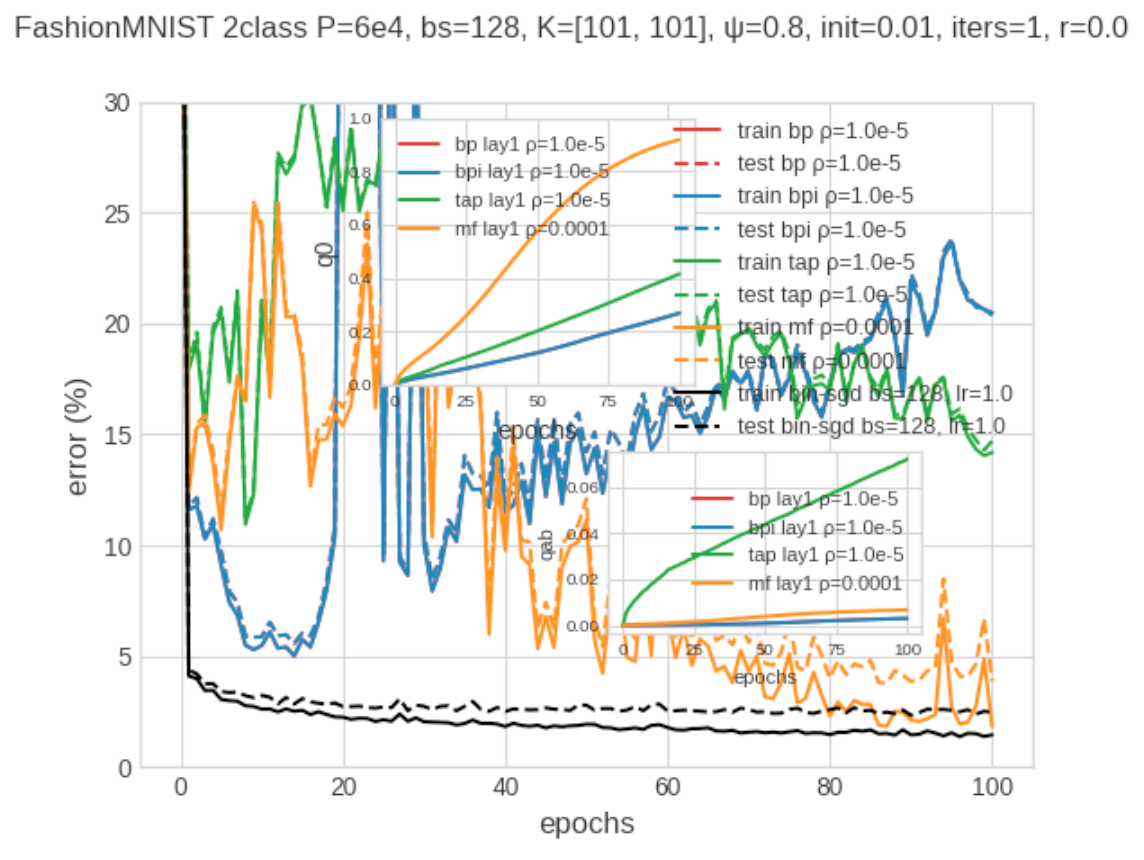
\includegraphics[scale=0.2]{figures/pasted_new/pasted4}

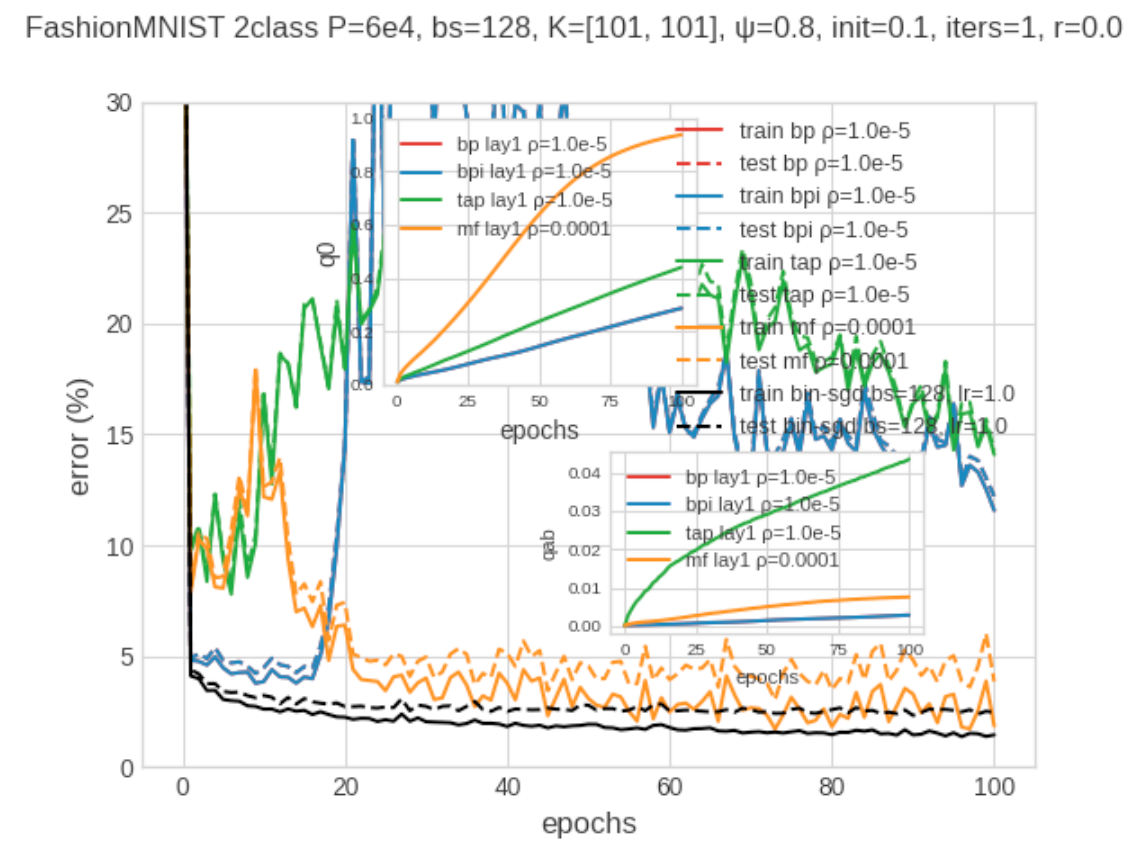
\includegraphics[scale=0.2]{figures/pasted_new/pasted7}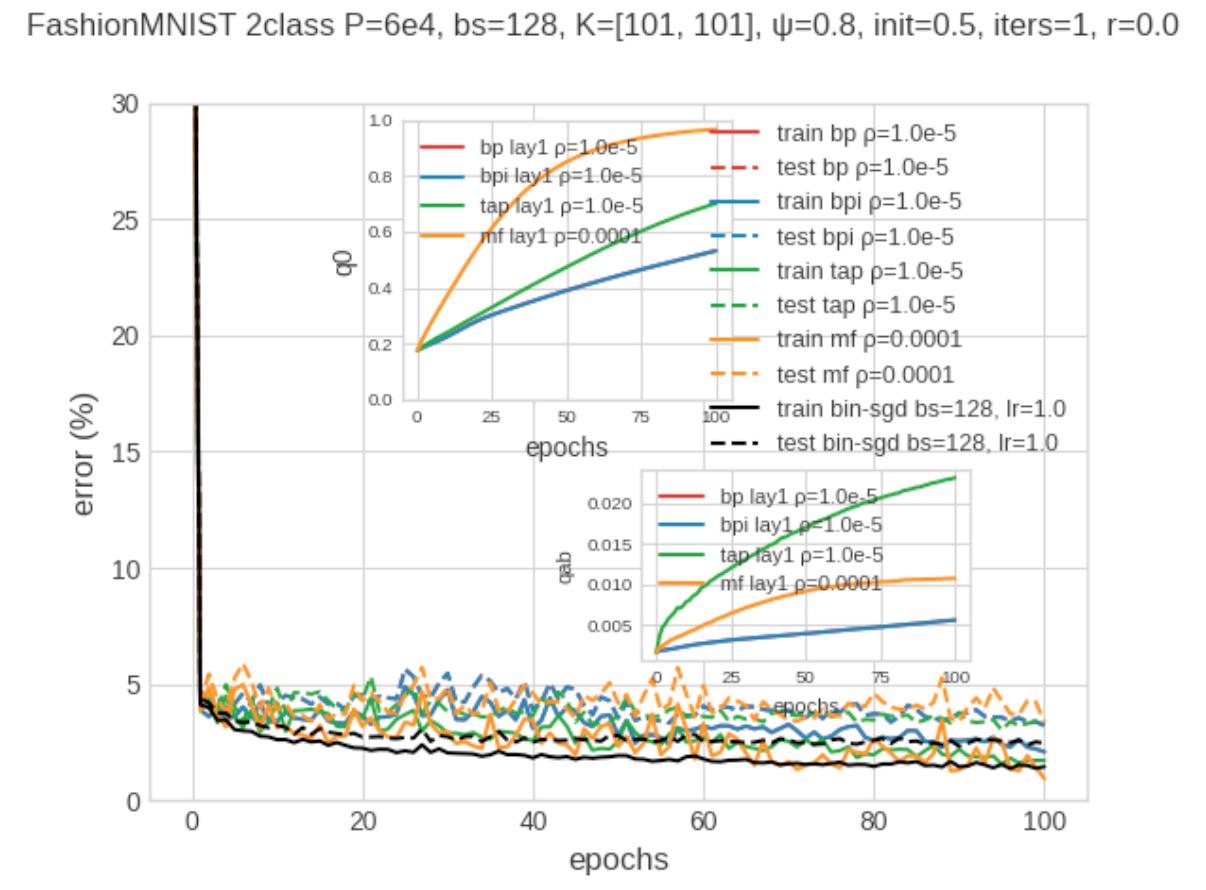
\includegraphics[scale=0.2]{figures/pasted_new/pasted8}

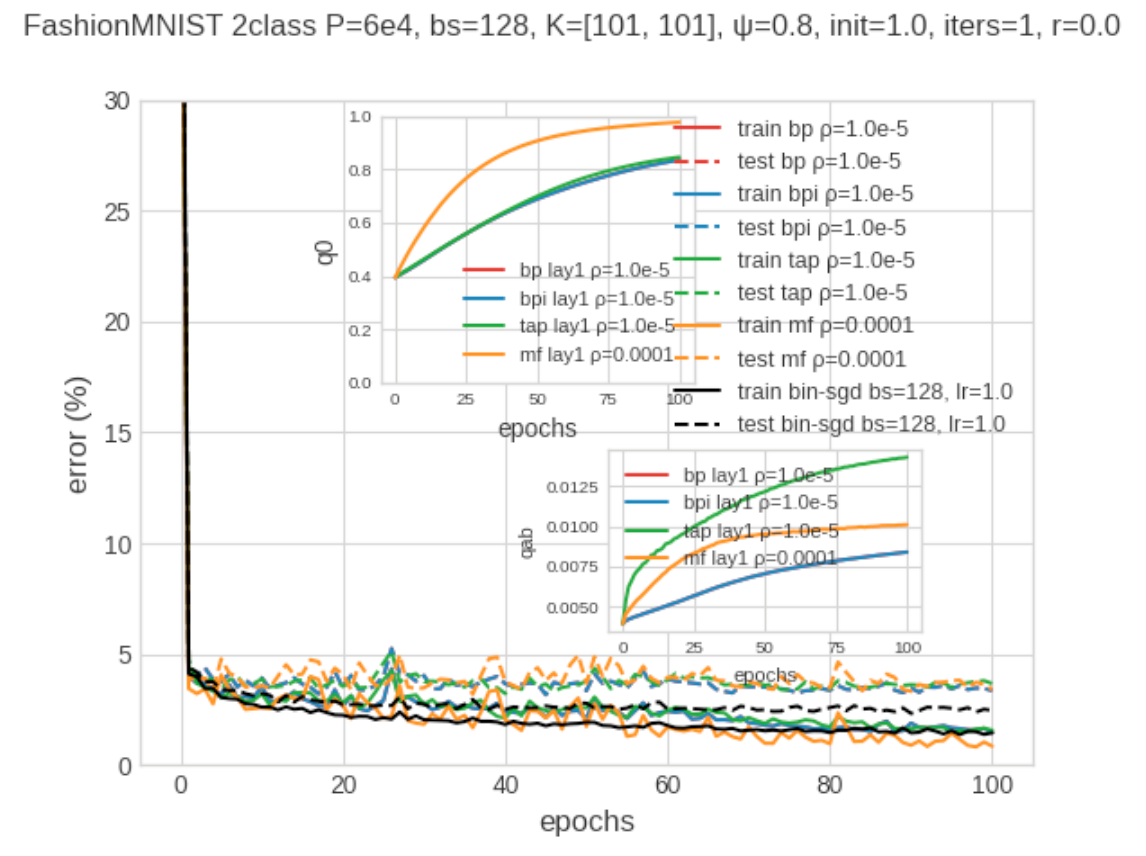
\includegraphics[scale=0.2]{figures/pasted_new/pasted1}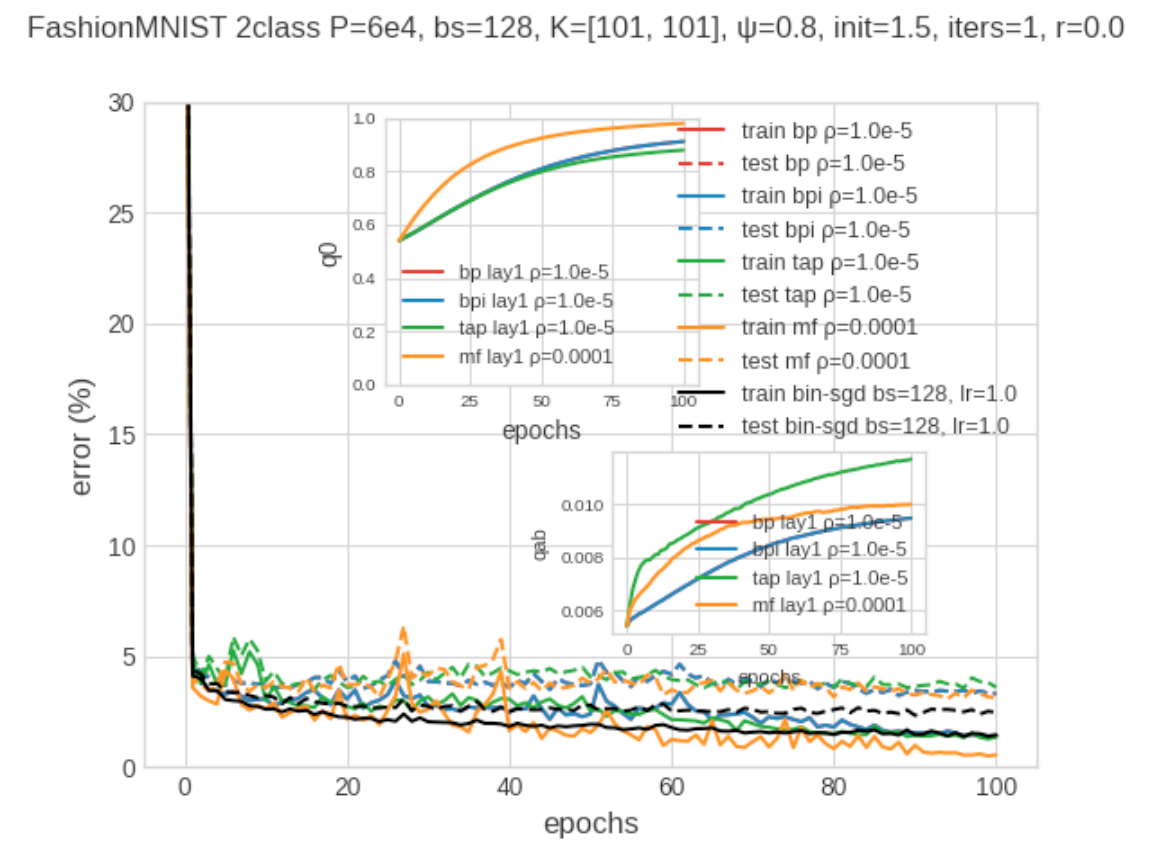
\includegraphics[scale=0.2]{figures/pasted_new/pasted2}

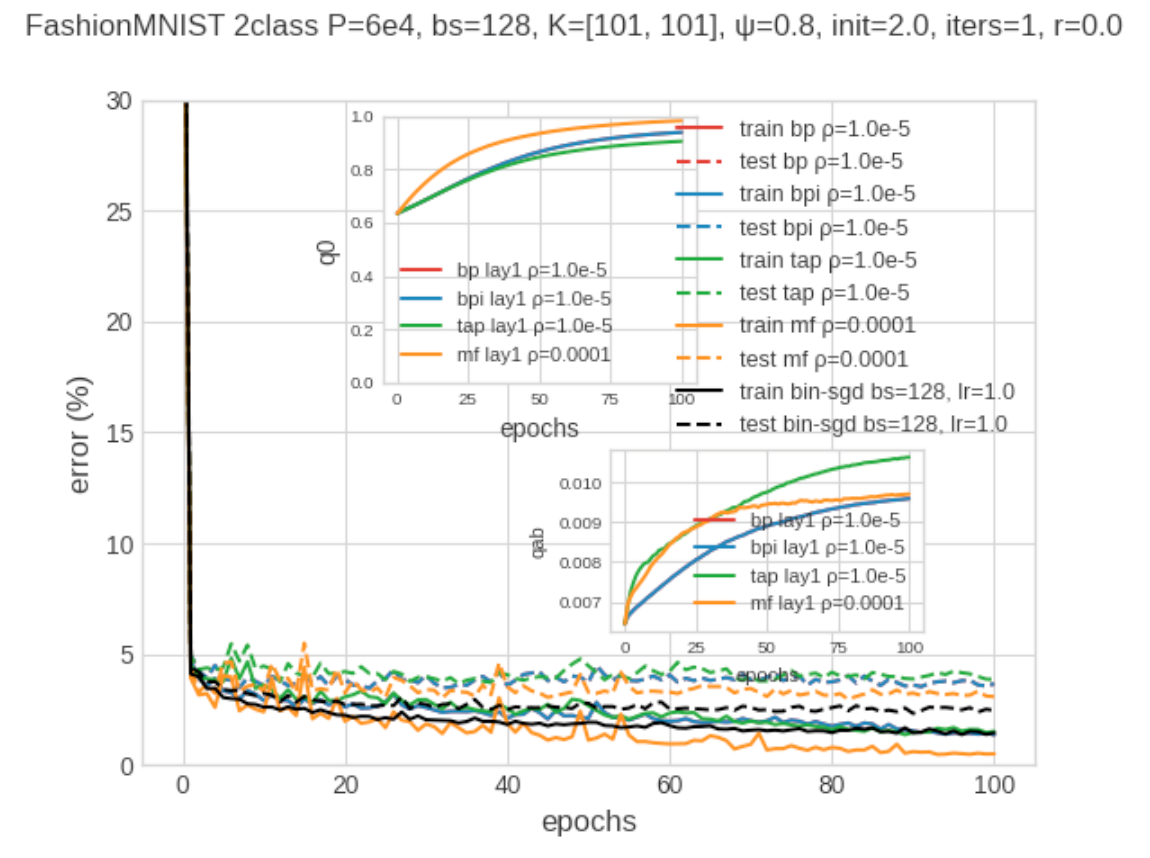
\includegraphics[scale=0.2]{figures/pasted_new/pasted3}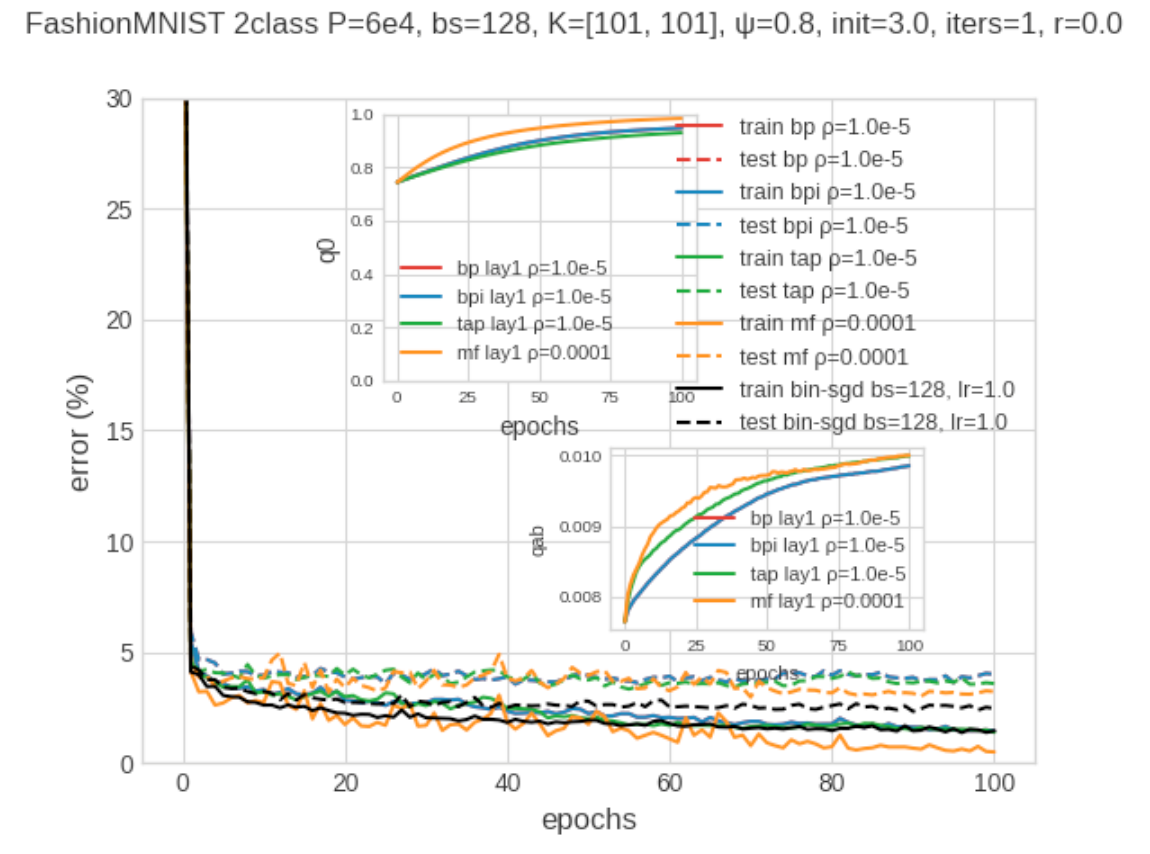
\includegraphics[scale=0.2]{figures/pasted_new/pasted5}

\caption{MLP with 2 hidden layers with 101 hidden units each, batch-size=128
on the Fashion-MNIST dataset. We vary the parameter $\epsilon$init.}
\end{figure}
\par\end{center}

\subsubsection{Varying damping $\psi$}

$\psi$s = {[}0:0.2:0.8;{]} $\cup$ {[}0.9, 0.99, 0.999, 0.9999{]}

For $bs=128$ and $\rho-1=10^{-4}$ we choose $\psi=0.8$. The command
is the same as the one in the first paragraph of section B except
for $\rho$ and $\psi$.
\begin{center}
\begin{figure}[H]
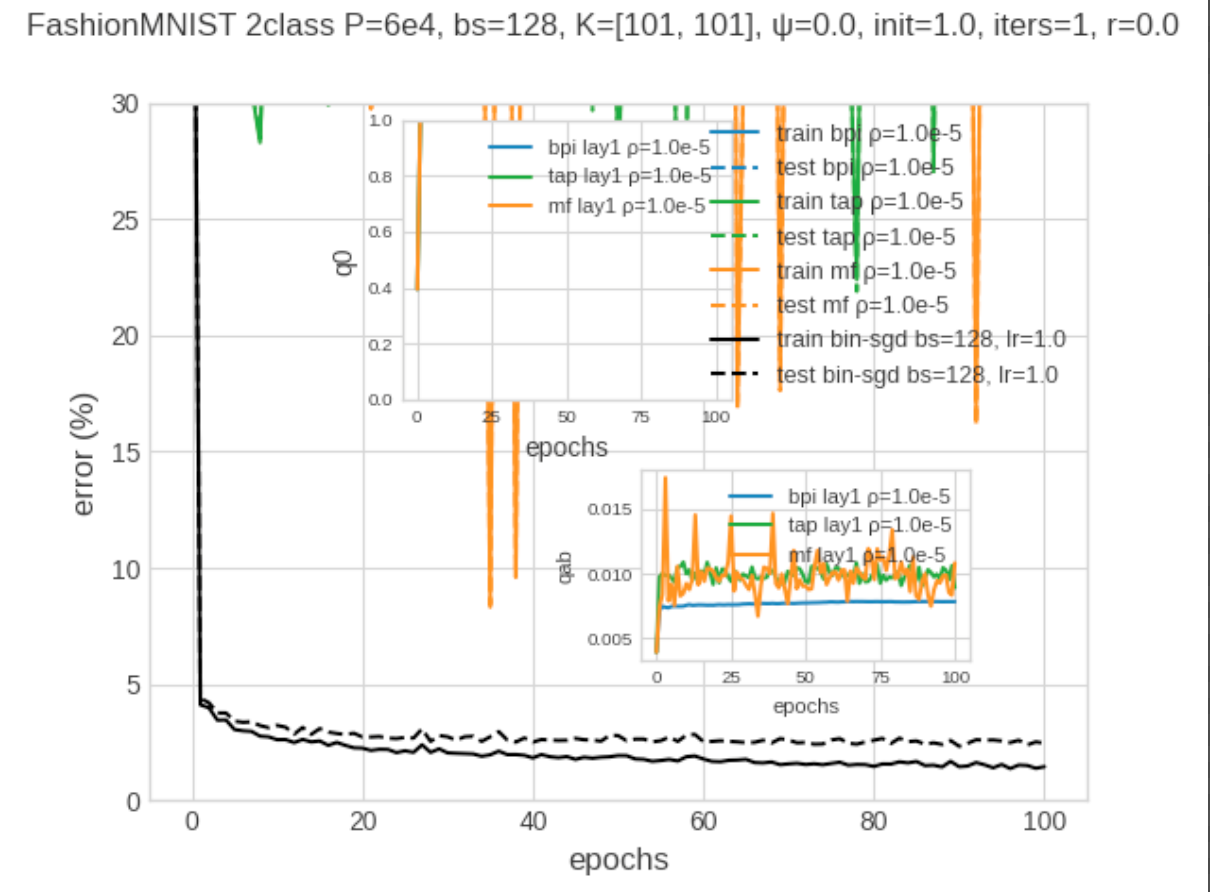
\includegraphics[scale=0.2]{figures/pasted_new/pasted17}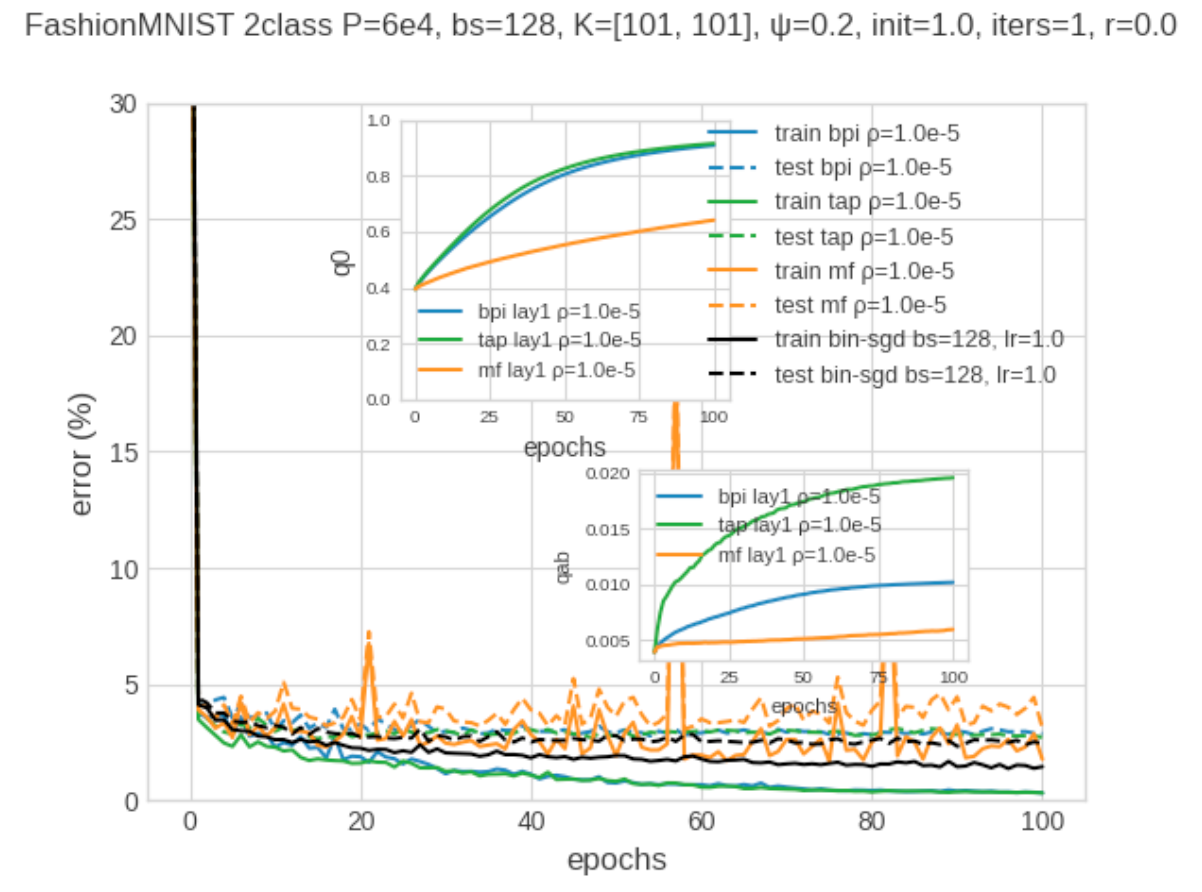
\includegraphics[scale=0.2]{figures/pasted_new/pasted18}

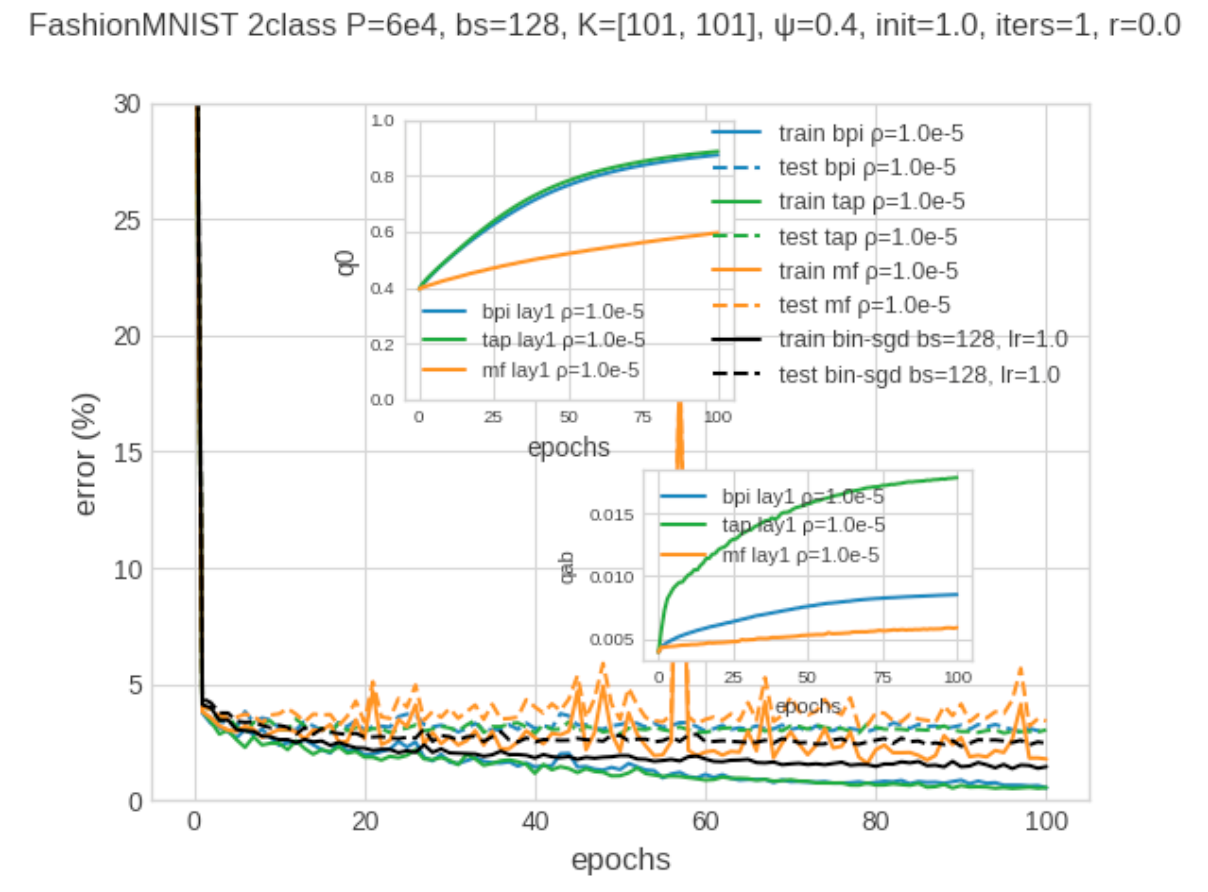
\includegraphics[scale=0.2]{figures/pasted_new/pasted19}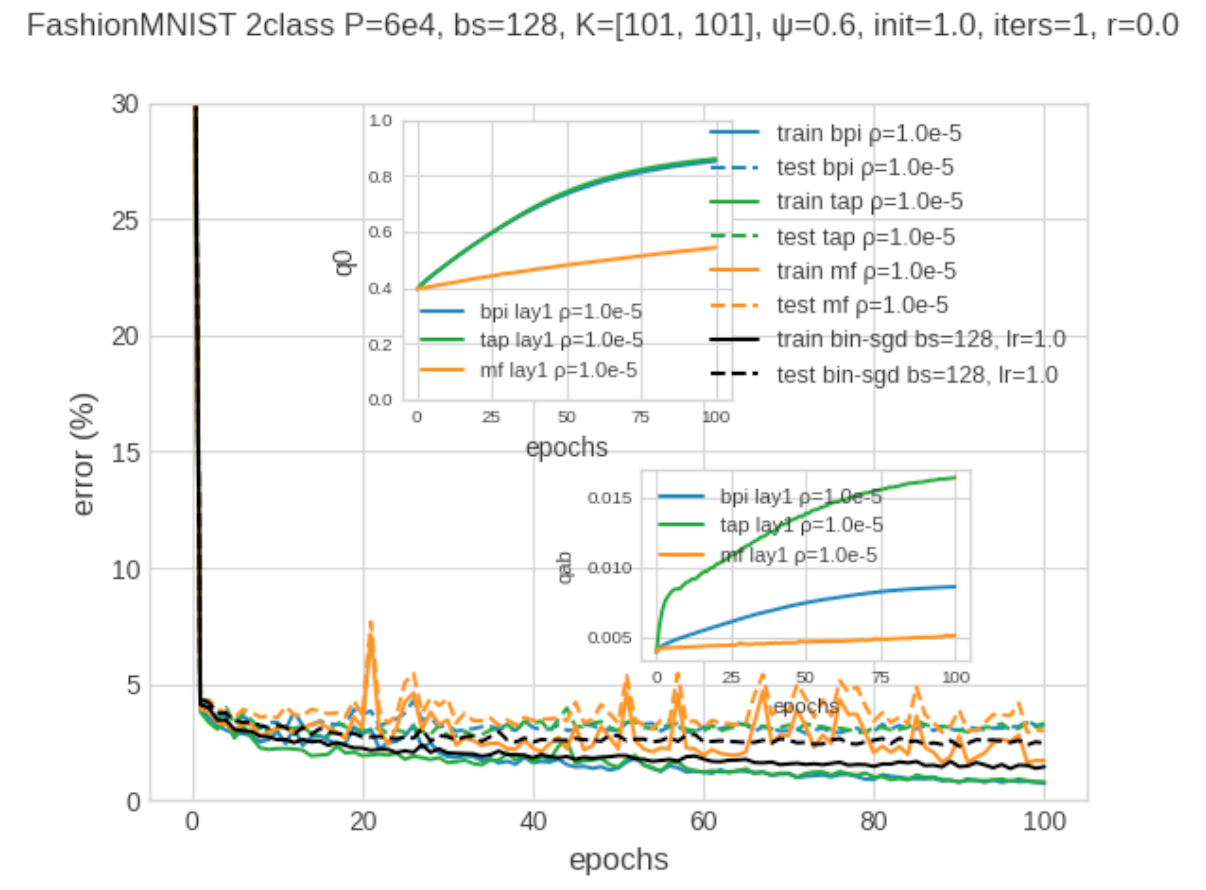
\includegraphics[scale=0.2]{figures/pasted_new/pasted20}

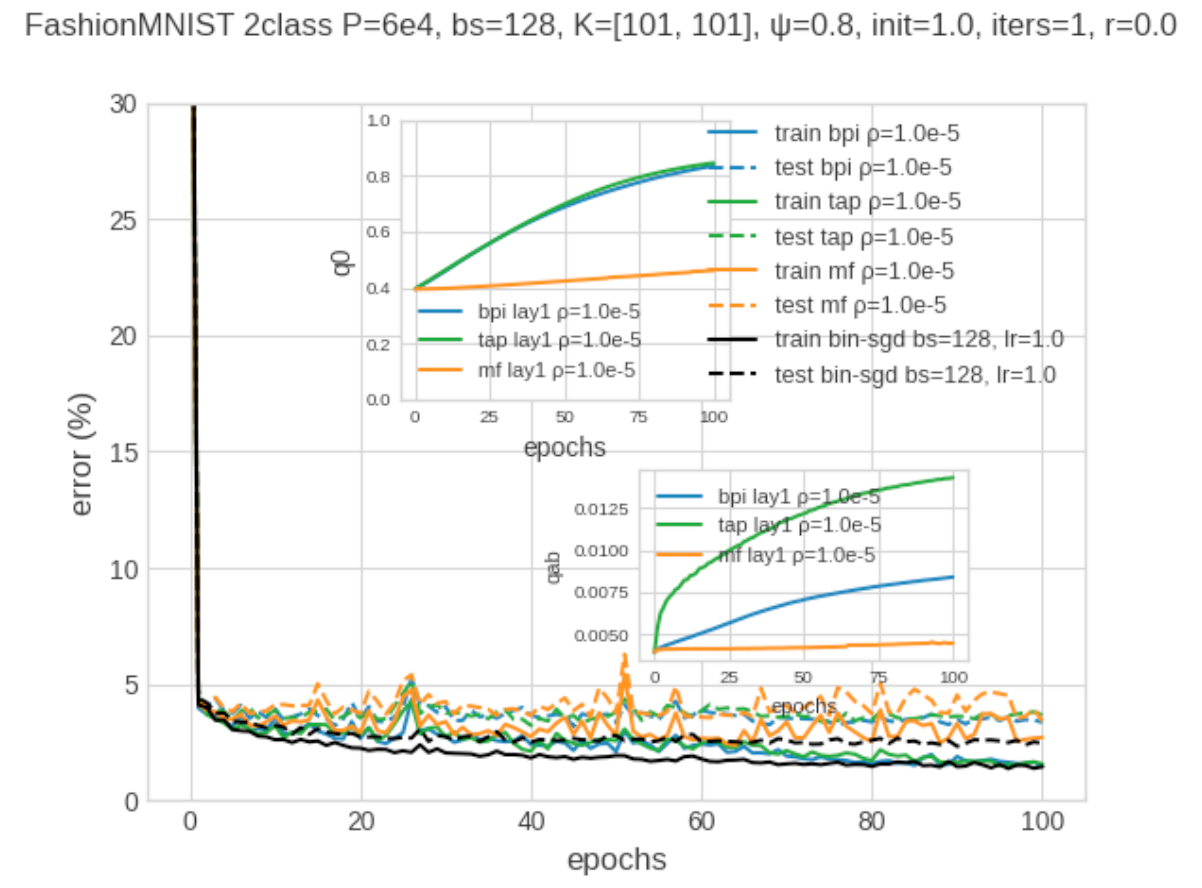
\includegraphics[scale=0.2]{figures/pasted_new/pasted21}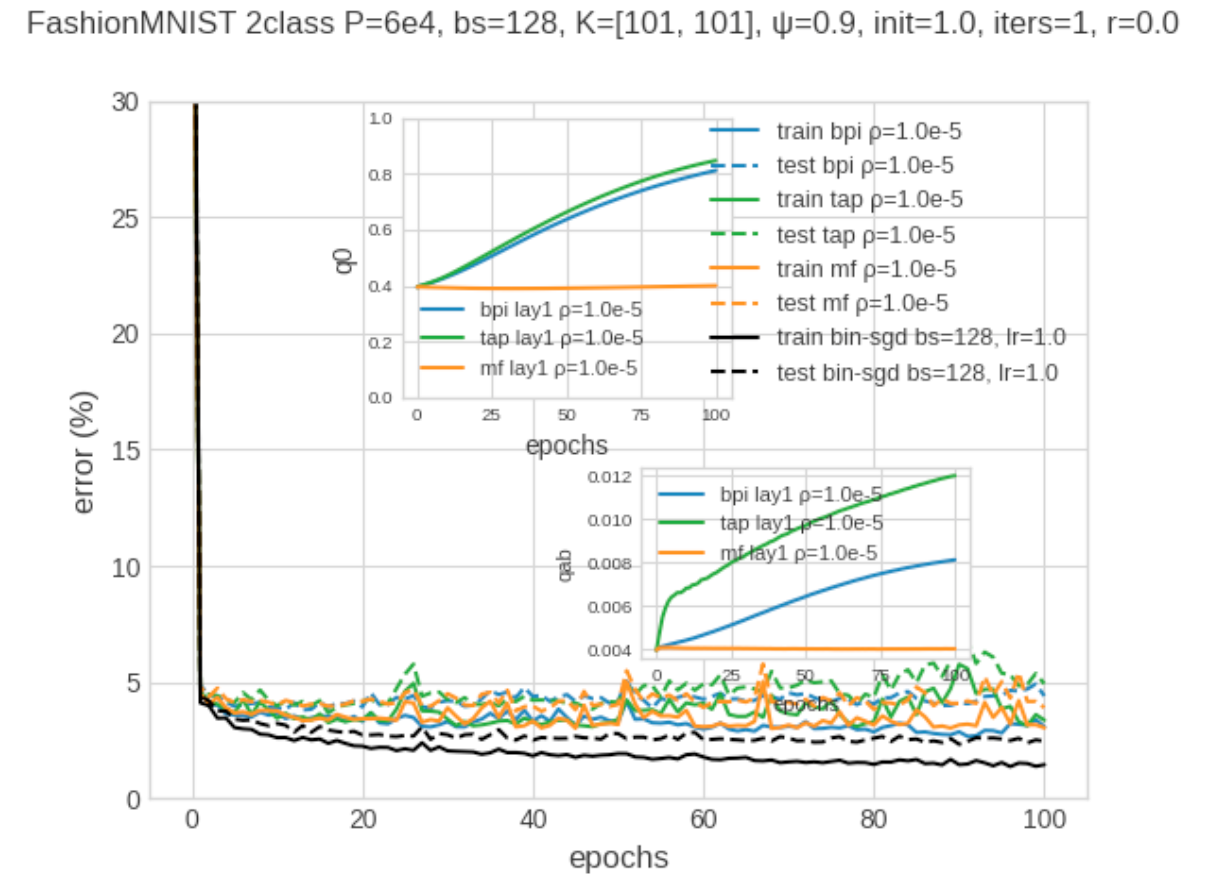
\includegraphics[scale=0.2]{figures/pasted_new/pasted22}

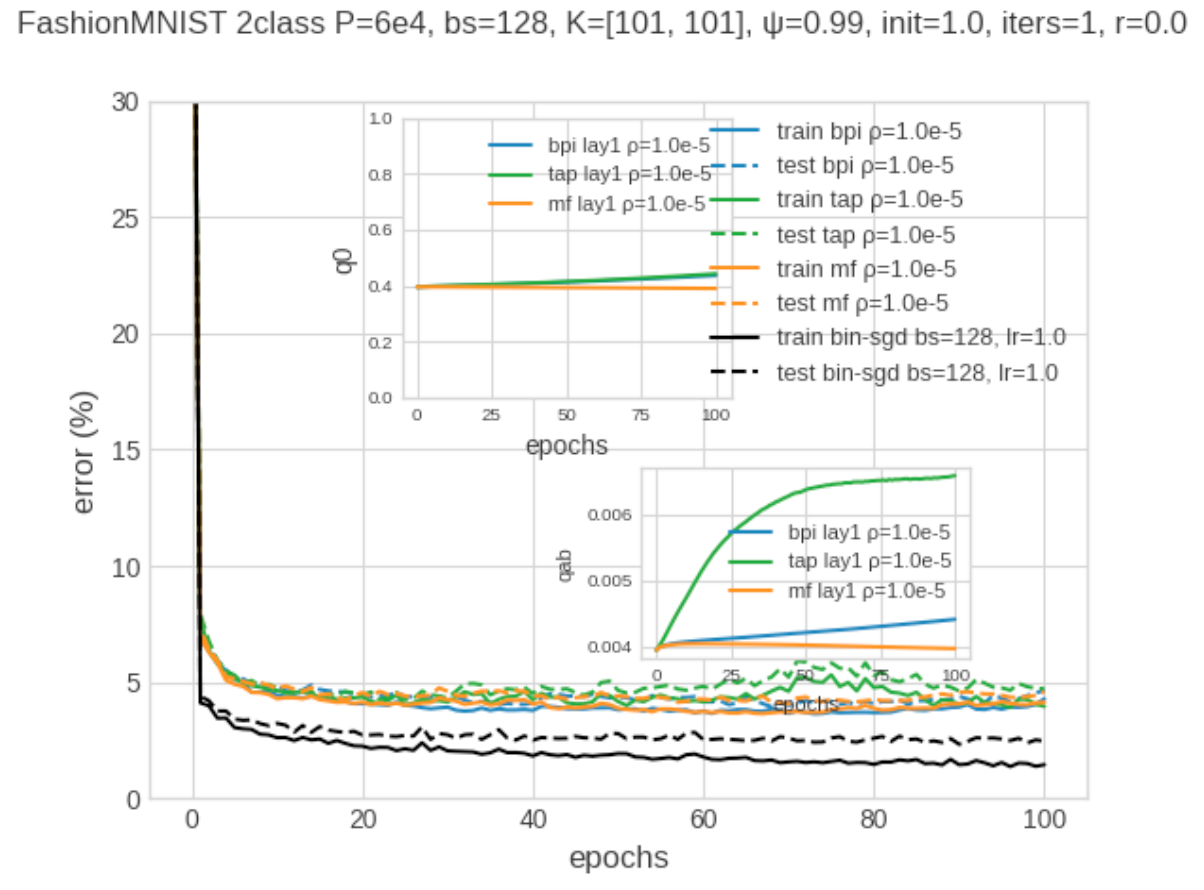
\includegraphics[scale=0.2]{figures/pasted_new/pasted23}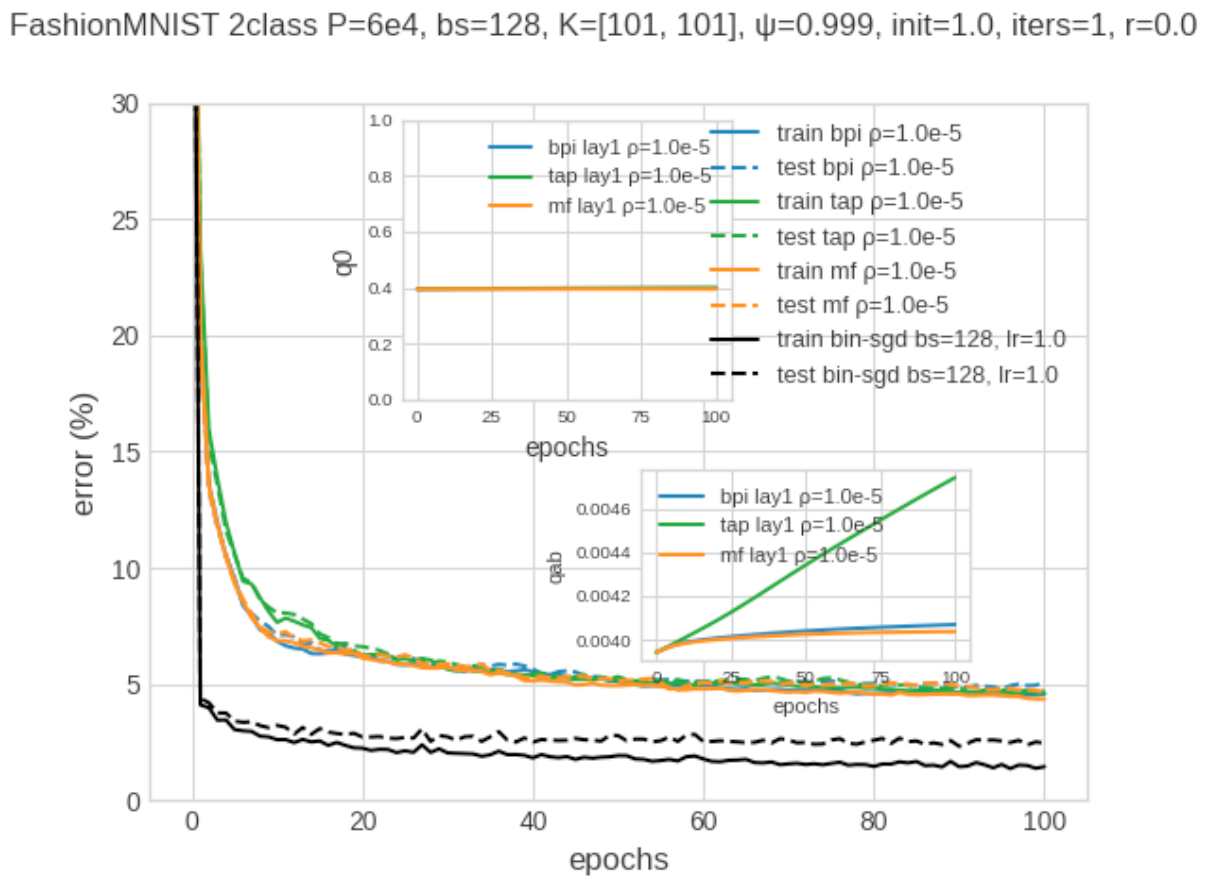
\includegraphics[scale=0.2]{figures/pasted_new/pasted24}

\caption{MLP with 2 hidden layers with 101 hidden units each, batch-size=128
on the Fashion-MNIST dataset. We vary the parameter $\psi$.}
\end{figure}
\par\end{center}

\subsubsection{Varying dataset size}

Ms = {[}Int(1e2), Int(1e3), Int(1e4), Int(6e4){]} 

bs = {[}Int(1e0), Int(1e1), Int(1e2), Int(6e2){]}

We fix the ratio $\frac{\text{dataset size}}{\text{batch size}}=\frac{M}{b}=10^{2}$.
\begin{center}
\begin{figure}[H]
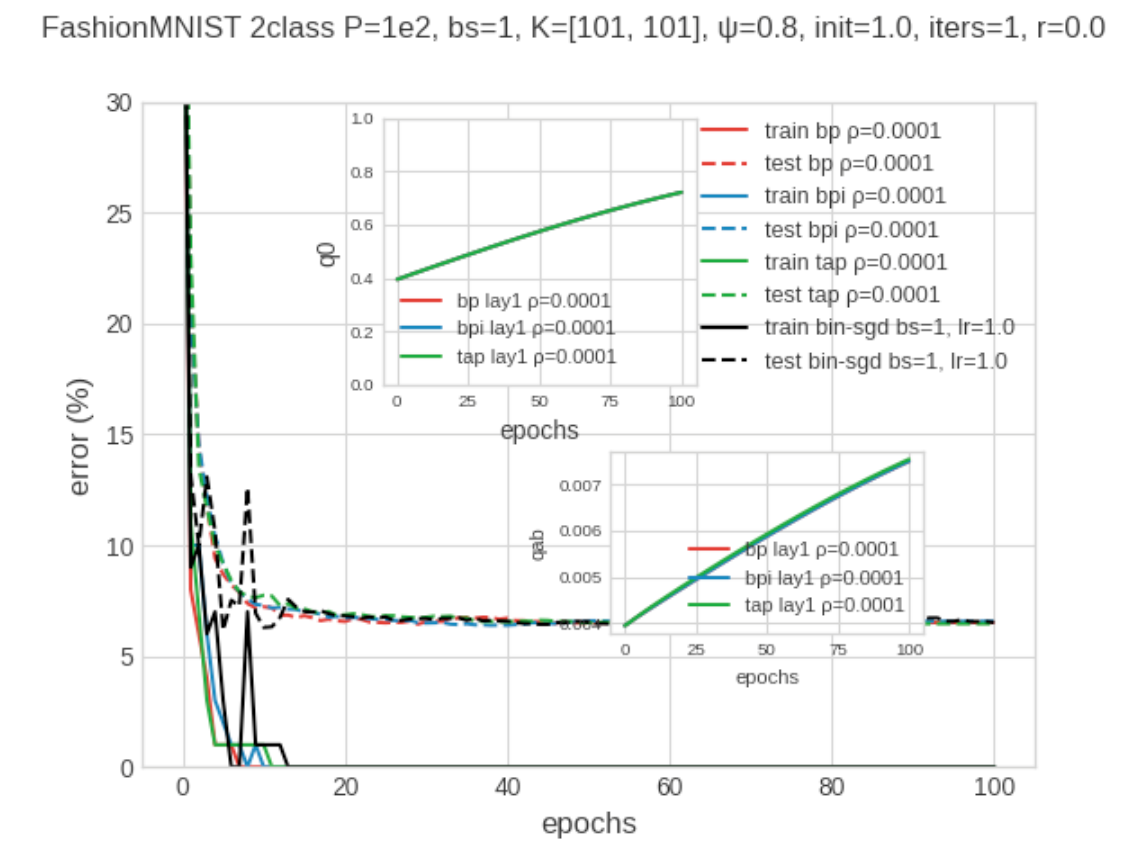
\includegraphics[scale=0.2]{figures/pasted/pasted51}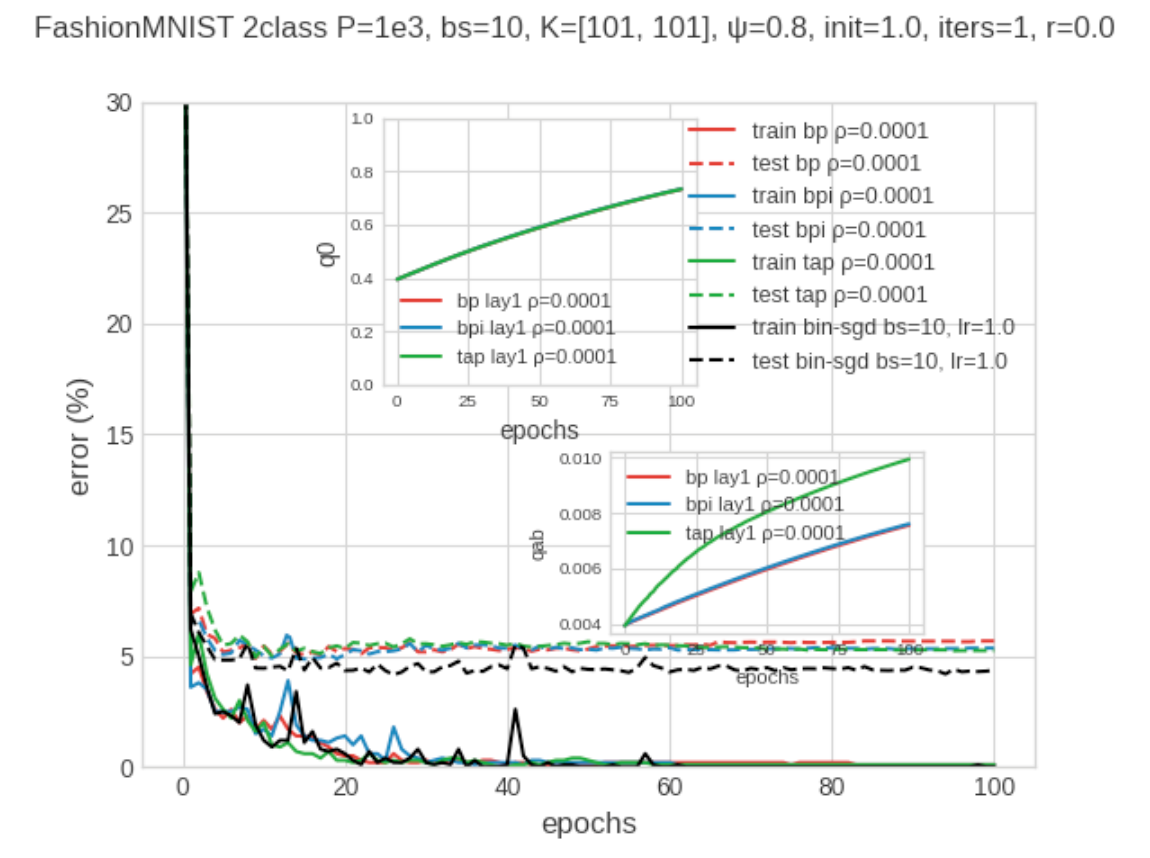
\includegraphics[scale=0.2]{figures/pasted/pasted52}

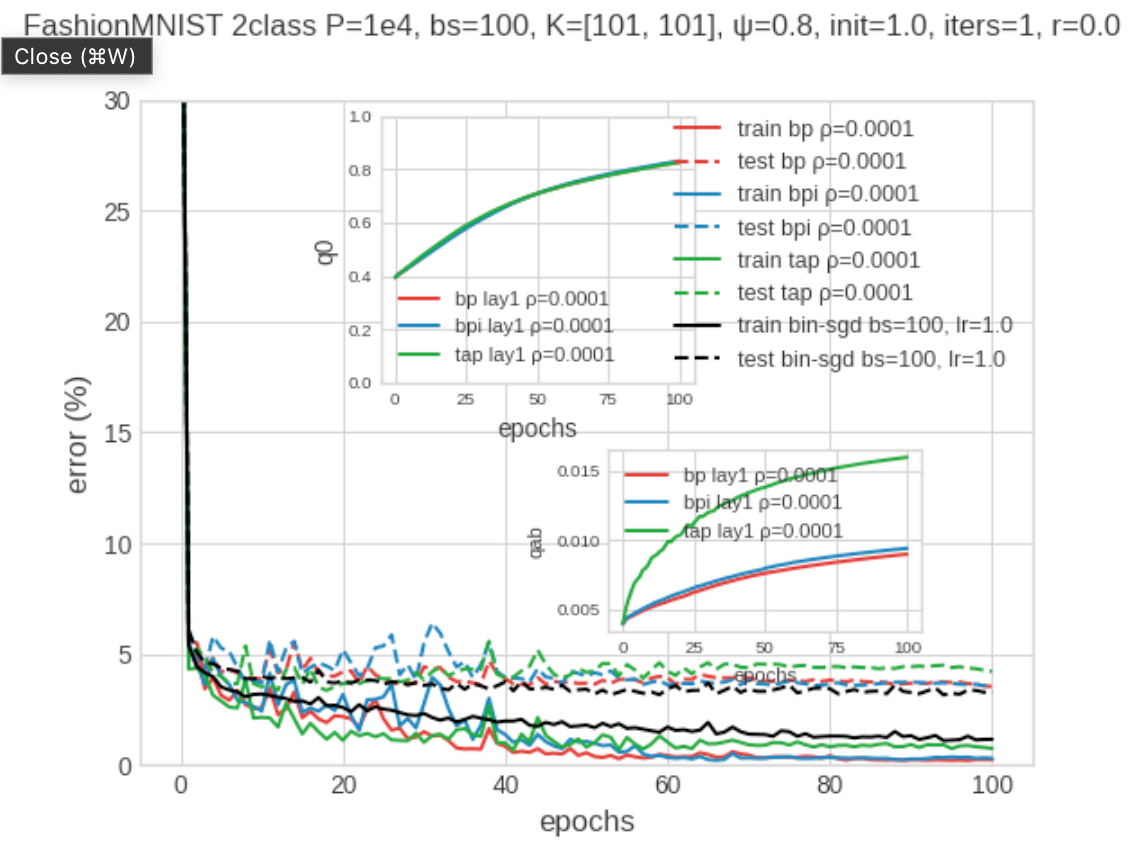
\includegraphics[scale=0.2]{figures/pasted/pasted49}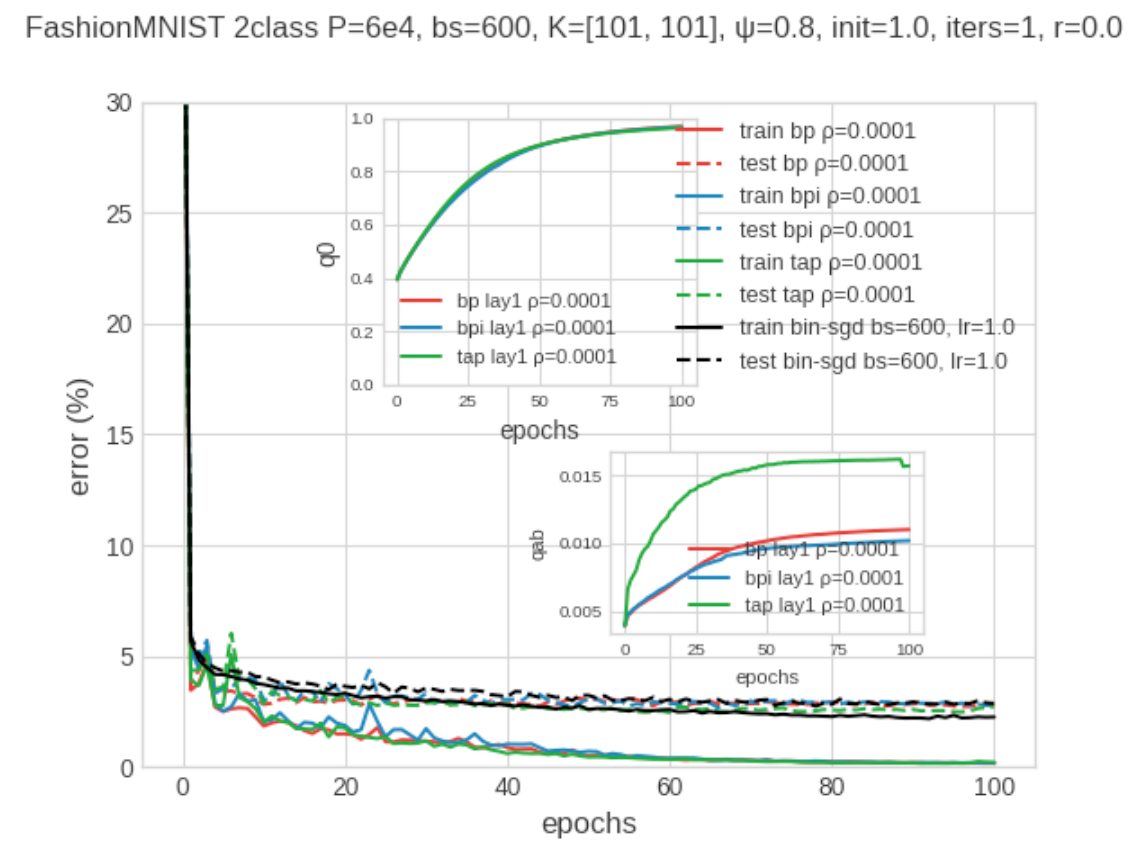
\includegraphics[scale=0.2]{figures/pasted/pasted50}

\caption{MLP with 2 hidden layers with 101 hidden units each, batch-size=128
on the Fashion-MNIST dataset. We vary the parameter $M$ (with $\frac{M}{b}=10^{2}$).}
\end{figure}
\par\end{center}

\subsubsection{Varying $maxiters$}

maxiterss = {[}1, 10, 50, 100{]}. Here also time is interesting. It
is not very favorable in terms of time compared to SGD to choose $maxiters>1$,
however it is interesting how many iterations are necessary for convergence.
\begin{center}
\begin{figure}[H]
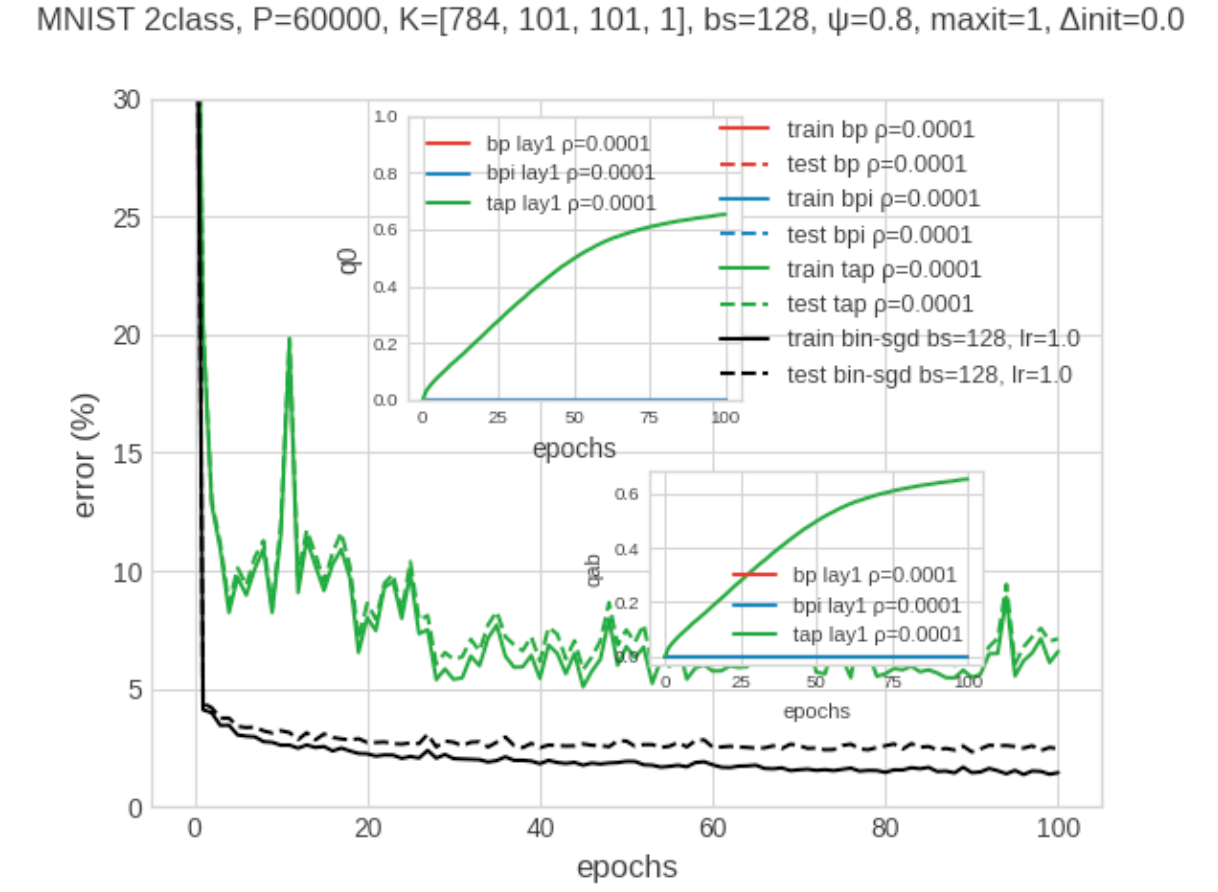
\includegraphics[scale=0.2]{figures/pasted/pasted39}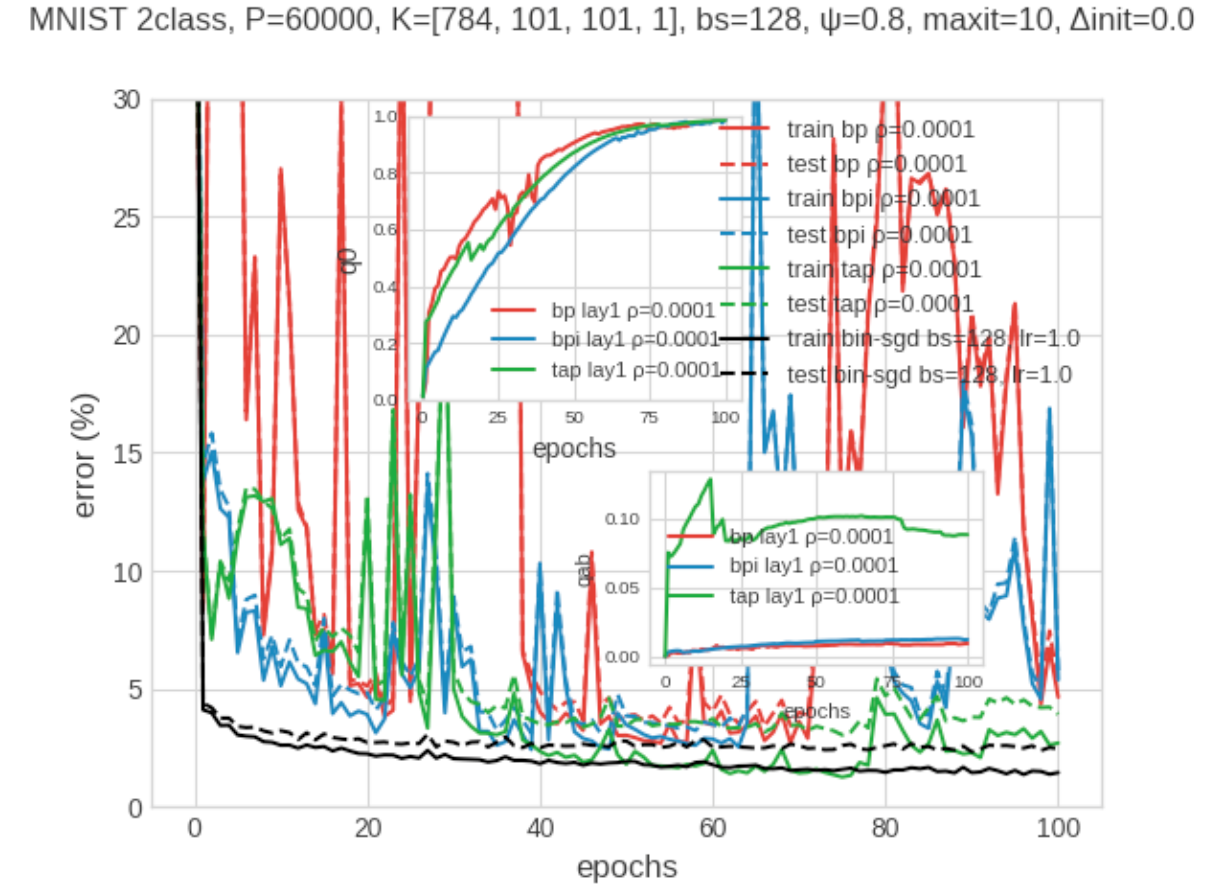
\includegraphics[scale=0.2]{figures/pasted/pasted40}

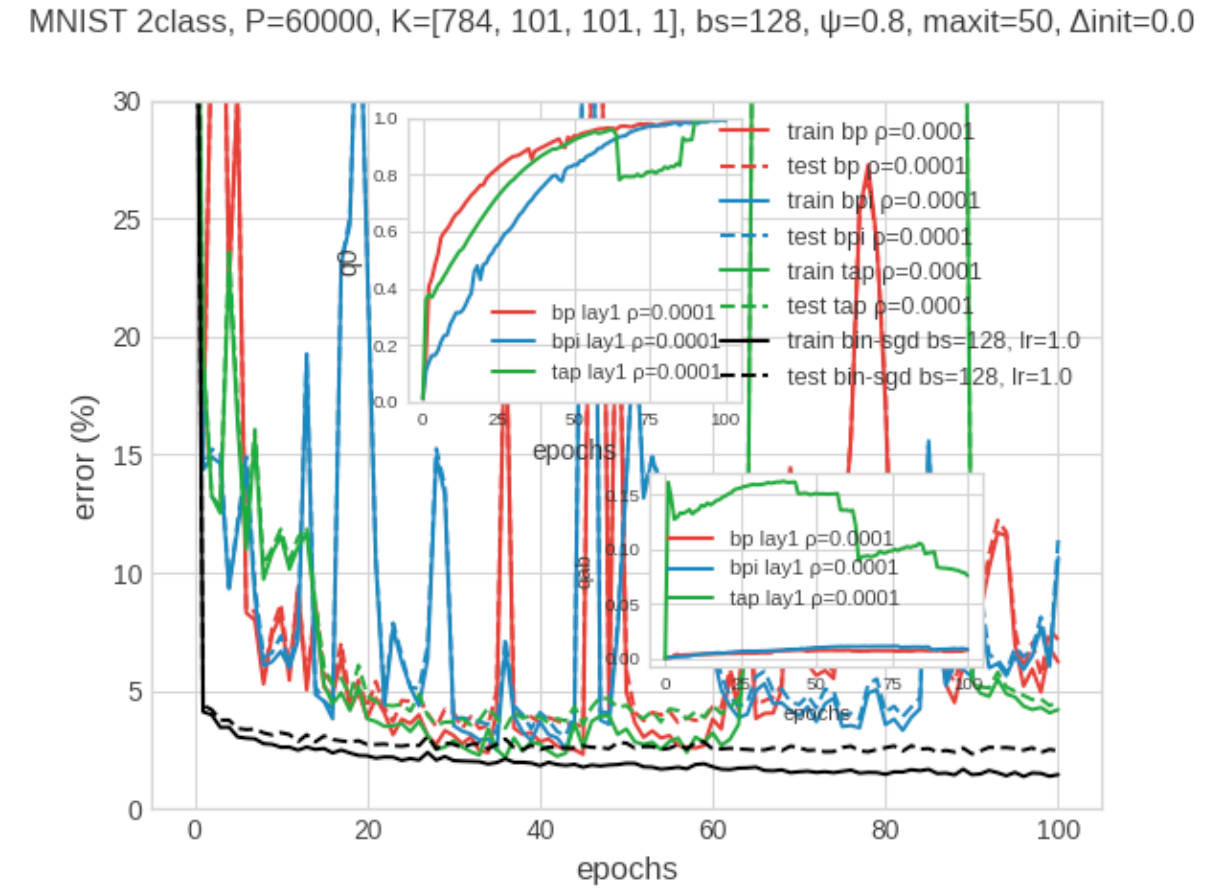
\includegraphics[scale=0.2]{figures/pasted/pasted41}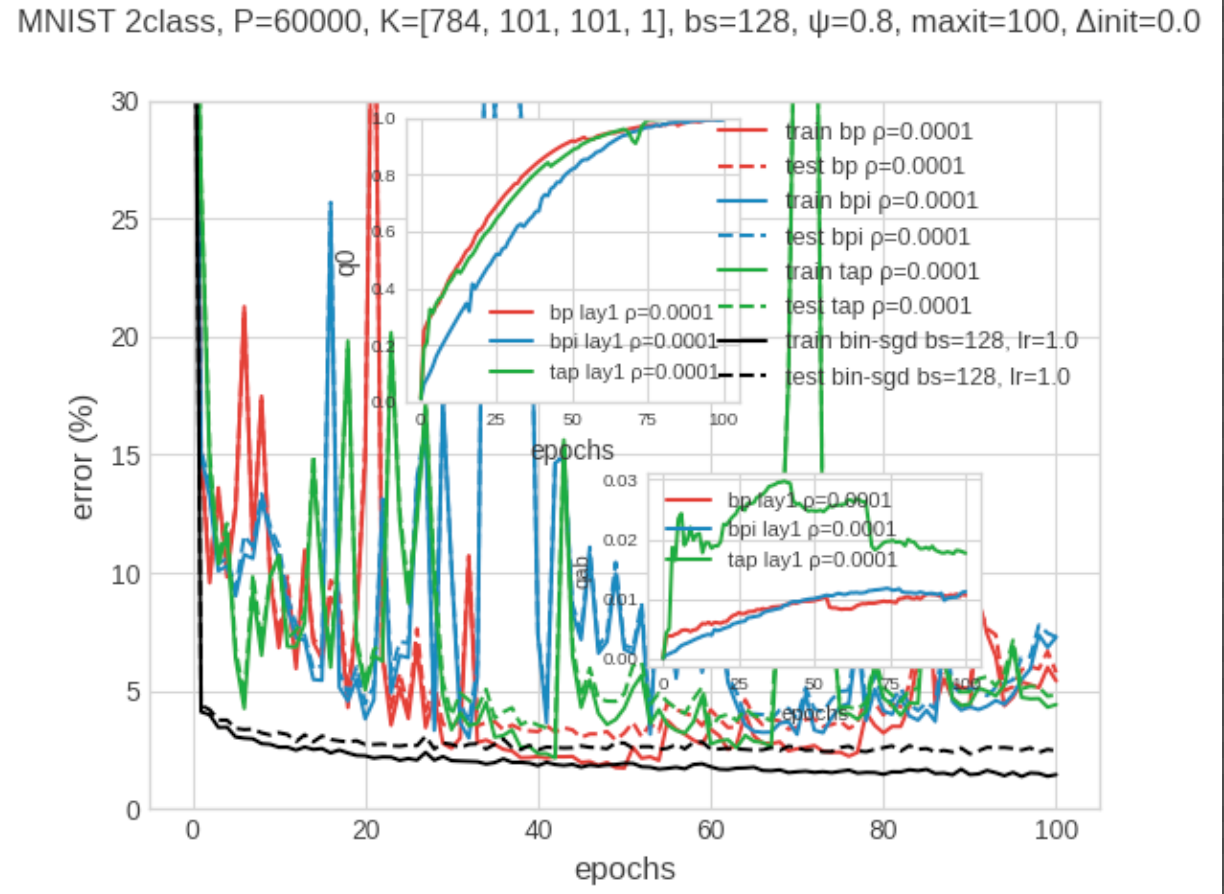
\includegraphics[scale=0.2]{figures/pasted/pasted42}

\caption{MLP with 2 hidden layers with 101 hidden units each, batch-size=128
on the Fashion-MNIST dataset. We vary the parameter $maxiters$.}
\end{figure}
\par\end{center}

\subsubsection{Varying $r$}

rs = {[}0:0.2:1.2;{]} (for maxiters=10). Da rifare.
\begin{center}
\begin{figure}[H]
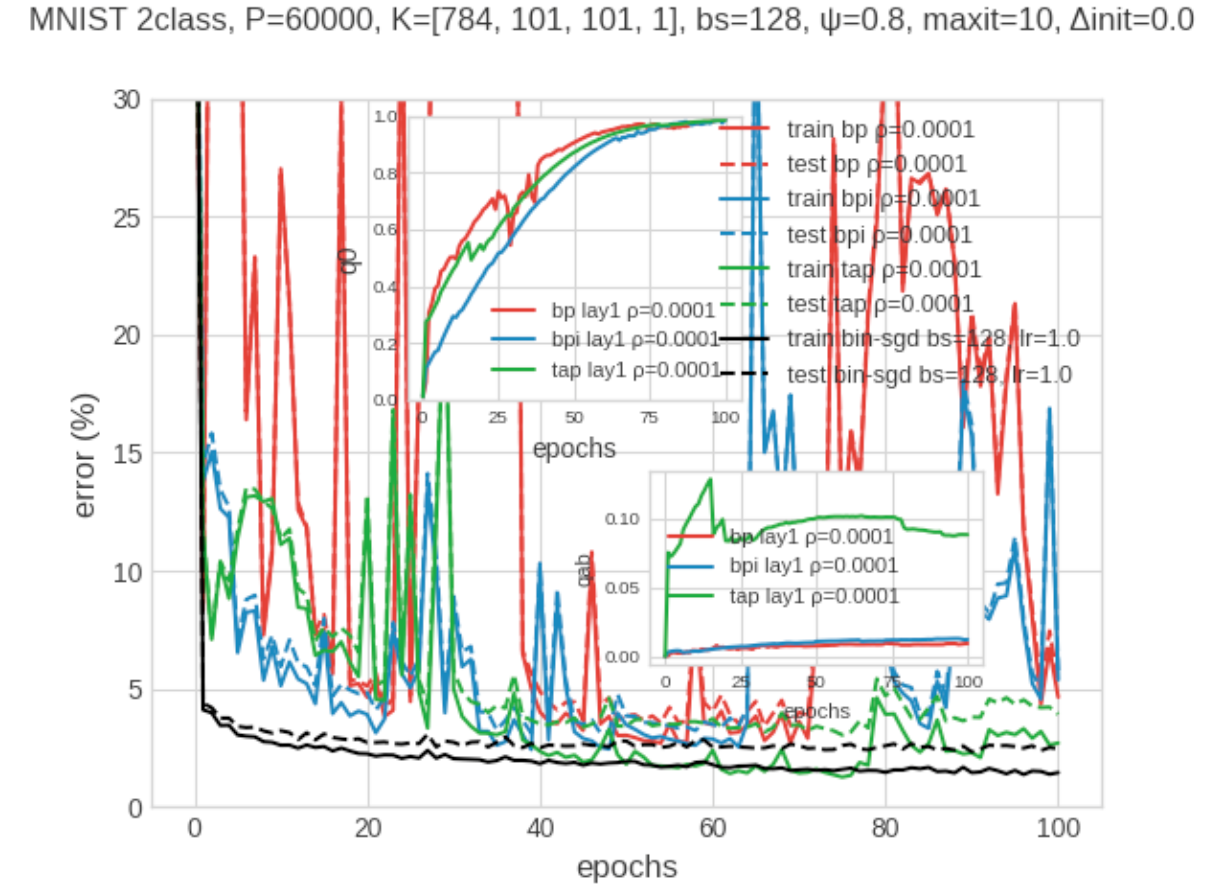
\includegraphics[scale=0.2]{figures/pasted/pasted40}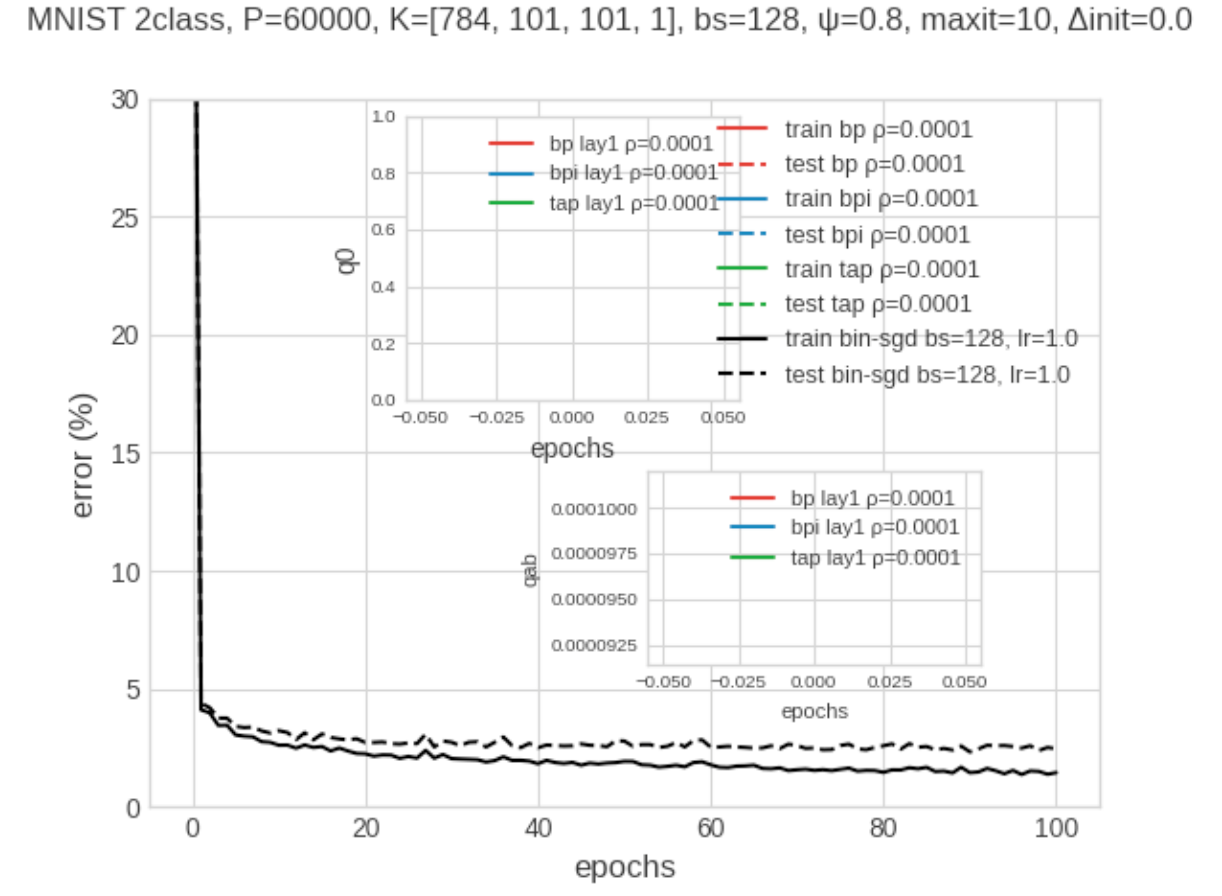
\includegraphics[scale=0.2]{figures/pasted/pasted43}

\caption{MLP with 2 hidden layers with 101 hidden units each, batch-size=128
on the Fashion-MNIST dataset. We fix $maxiters=10$ (just to be faster)
and we vary the parameter $r$. I vari valori di $r\protect\ne0$
non hanno proprio funzionato (sembra siano tutti NaN) - gli altri
parametri vanno cambiati.}
\end{figure}
\par\end{center}

\subsubsection{Varying the number of layers and the size of the hidden layer}

We fix some reasonable values of the hyperparameters (see previous
experiments, in particular: $P=6e4$, $bs=128$, $\psi=0.8$, $\epsilon init=1$,
$maxiters=1$, $r=0$) and want to check if the algorithm converges
(and todo the time scaling).
\begin{center}
\begin{figure}[H]
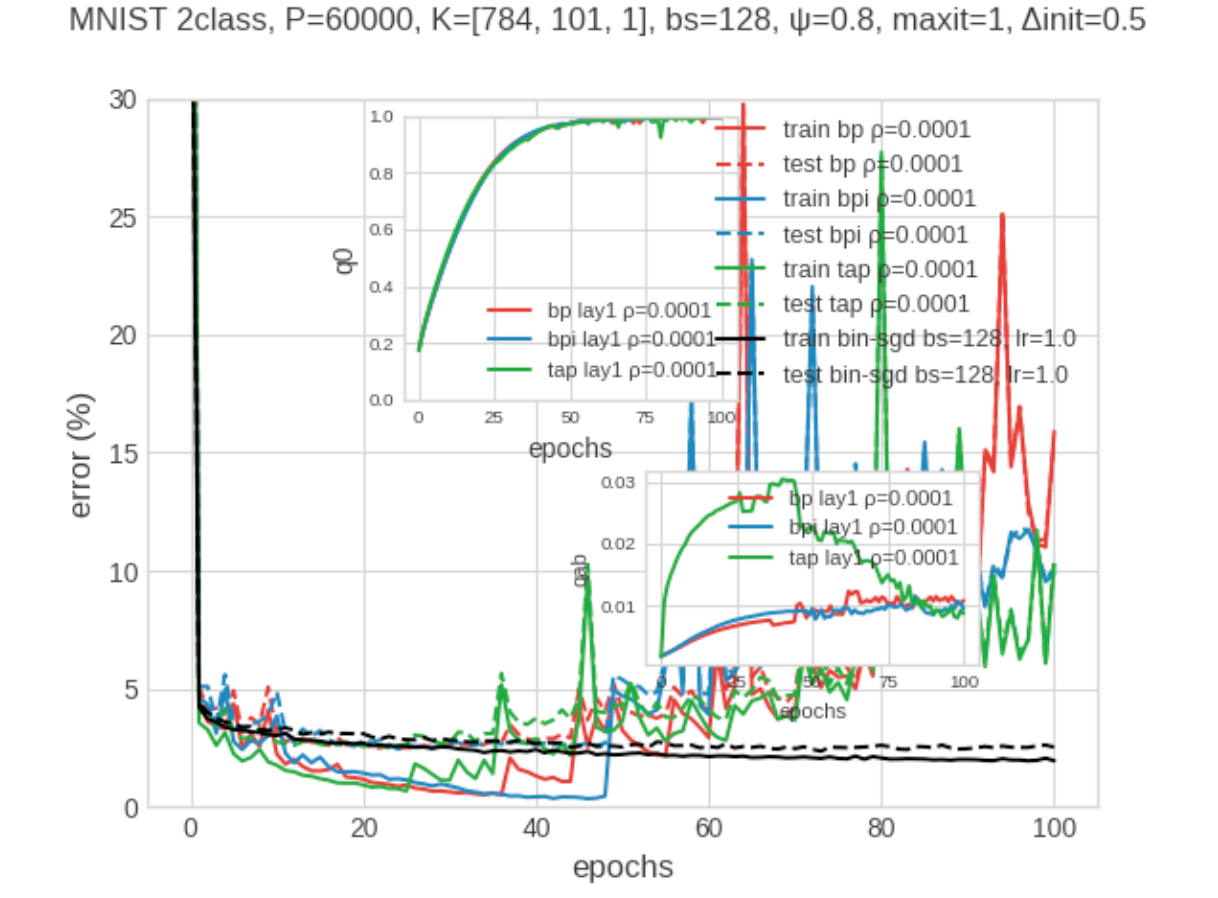
\includegraphics[scale=0.2]{figures/pasted/pasted26}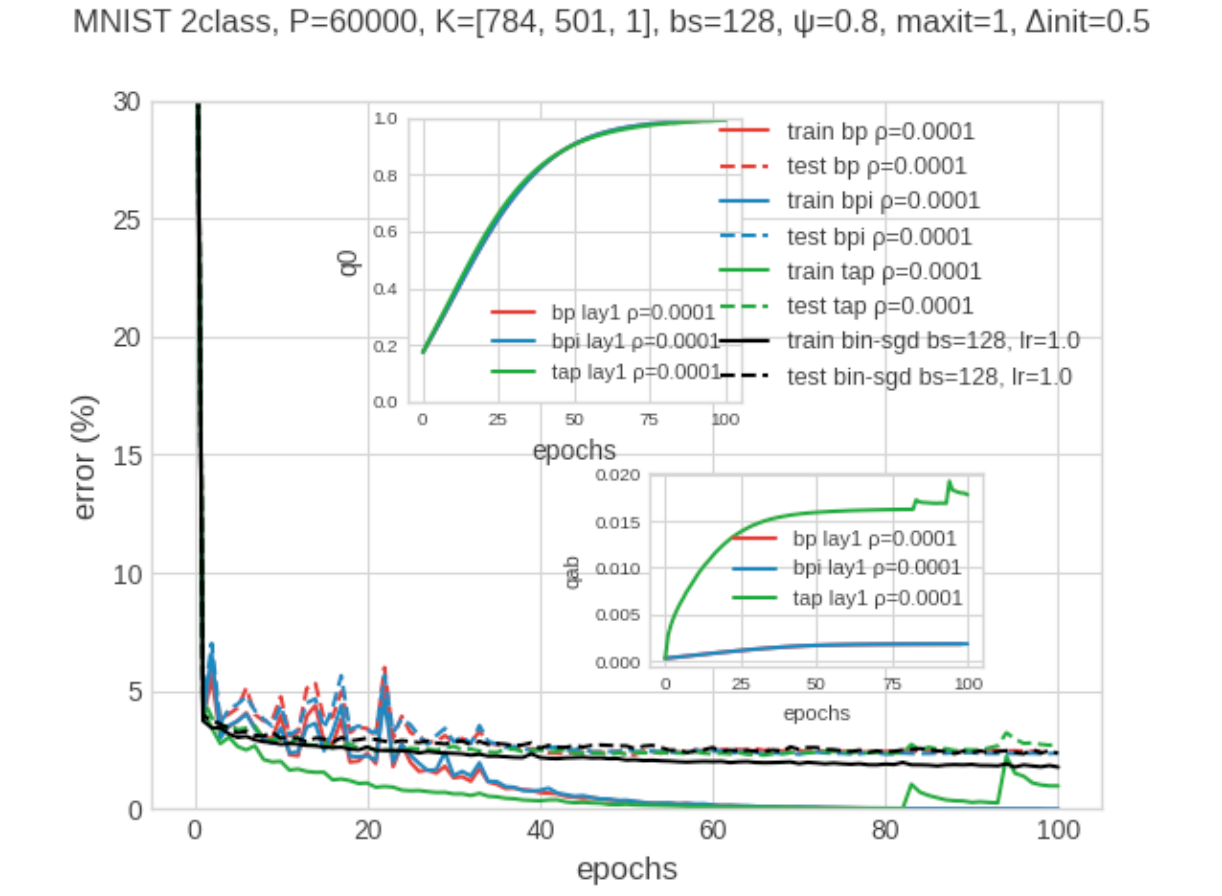
\includegraphics[scale=0.2]{figures/pasted/pasted27}

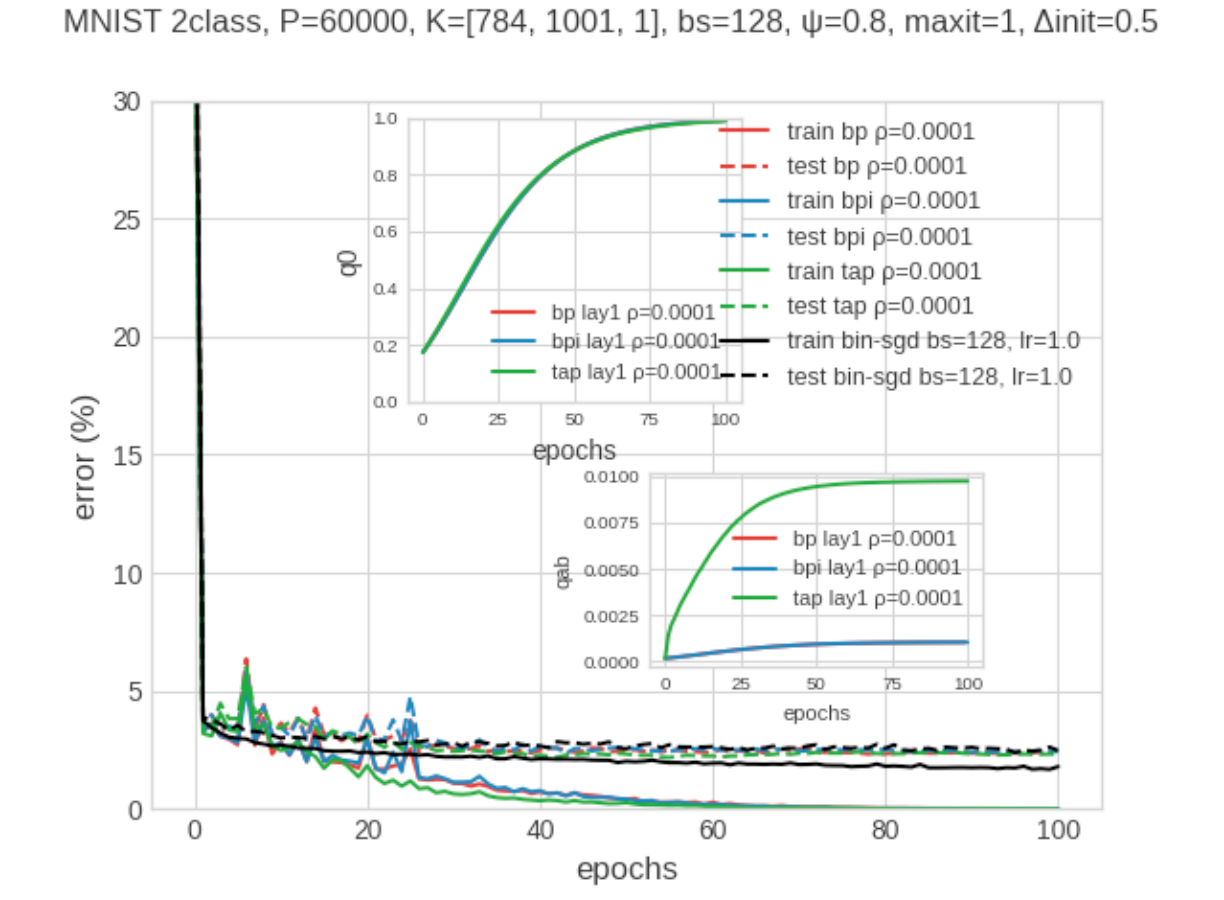
\includegraphics[scale=0.2]{figures/pasted/pasted28}

\caption{MLP with 1 hidden layer with 101/501/1001 hidden units each, batch-size=128
on the Fashion-MNIST dataset.}
\end{figure}
\par\end{center}

\begin{center}
\begin{figure}[H]
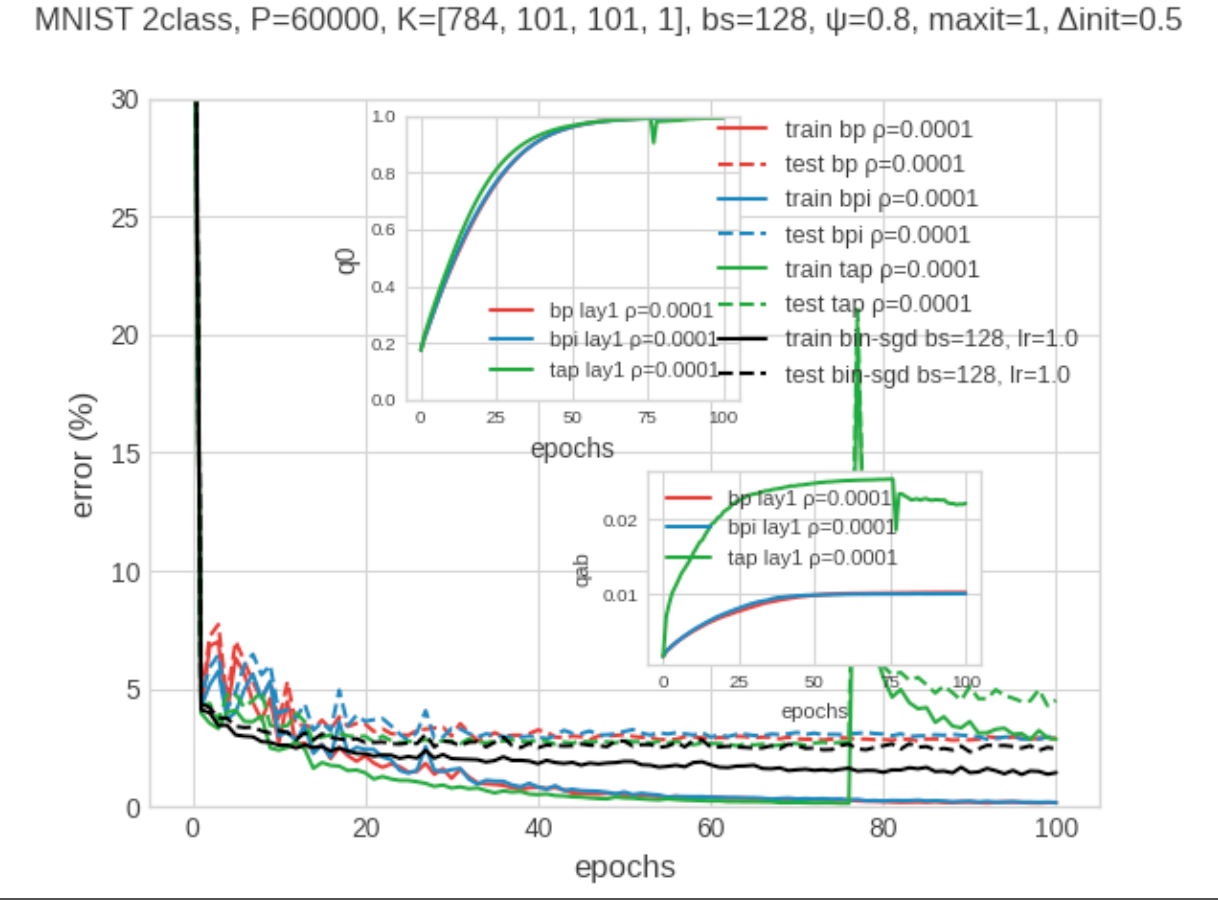
\includegraphics[scale=0.2]{figures/pasted/pasted29}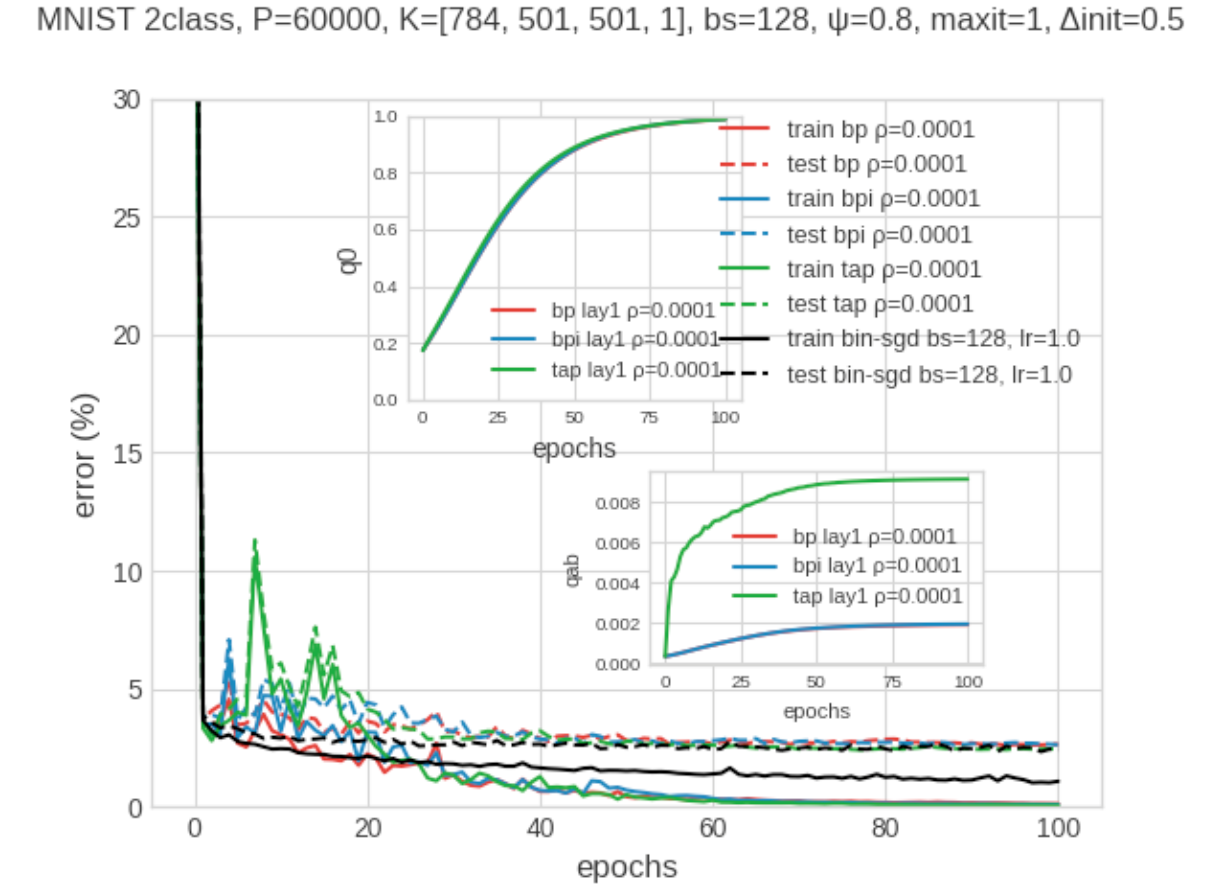
\includegraphics[scale=0.2]{figures/pasted/pasted30}

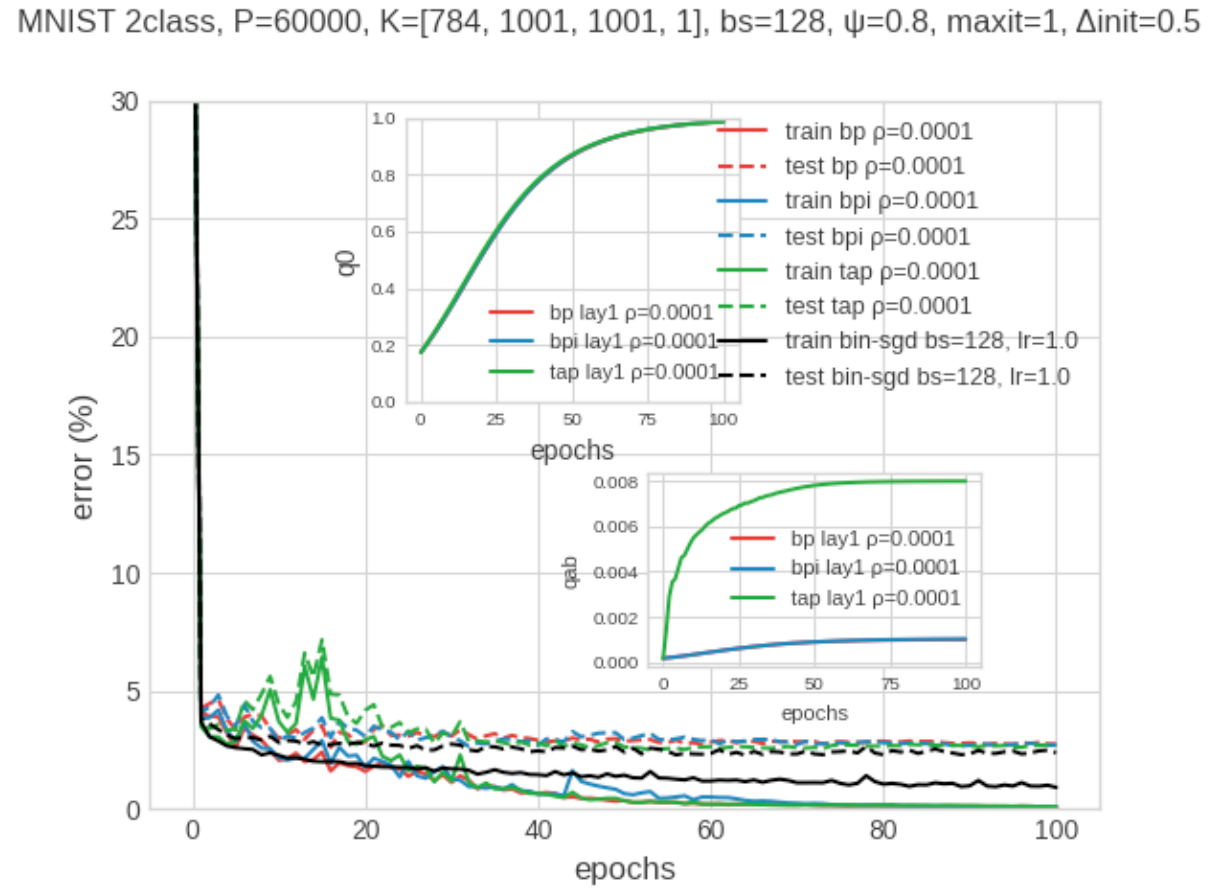
\includegraphics[scale=0.2]{figures/pasted/pasted31}

\caption{MLP with 2 hidden layers with 101/501/1001 hidden units each, batch-size=128
on the Fashion-MNIST dataset.}
\end{figure}
\par\end{center}

\begin{center}
\begin{figure}[H]
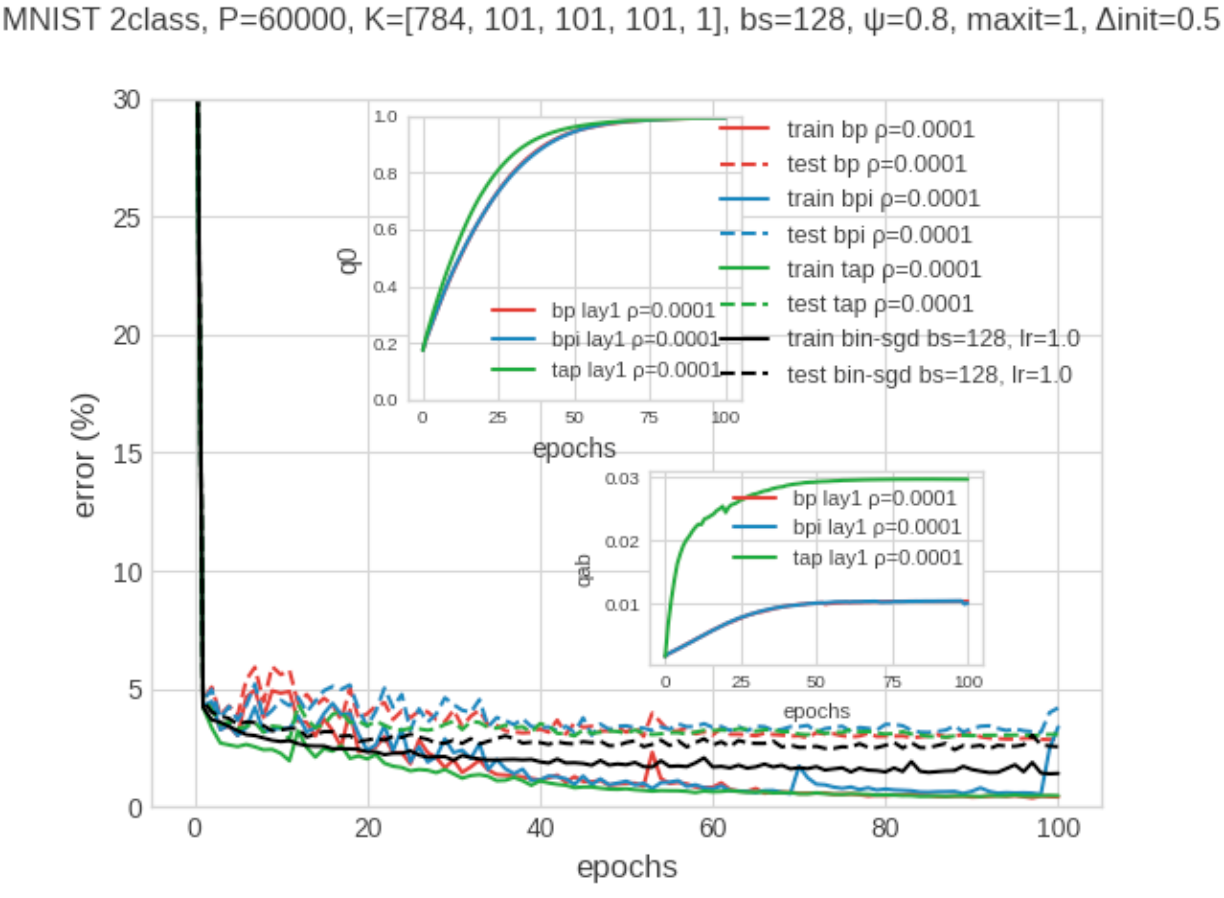
\includegraphics[scale=0.2]{figures/pasted/pasted32}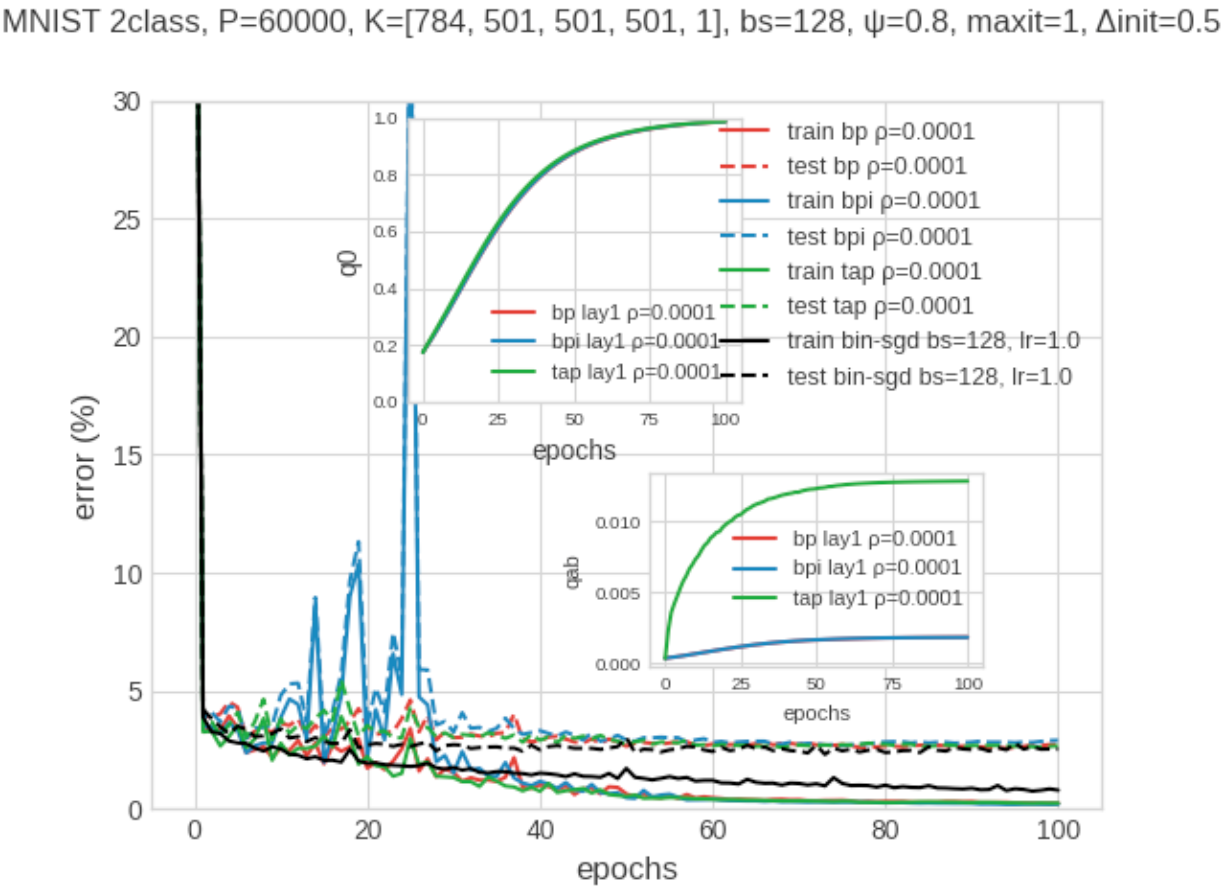
\includegraphics[scale=0.2]{figures/pasted/pasted33}

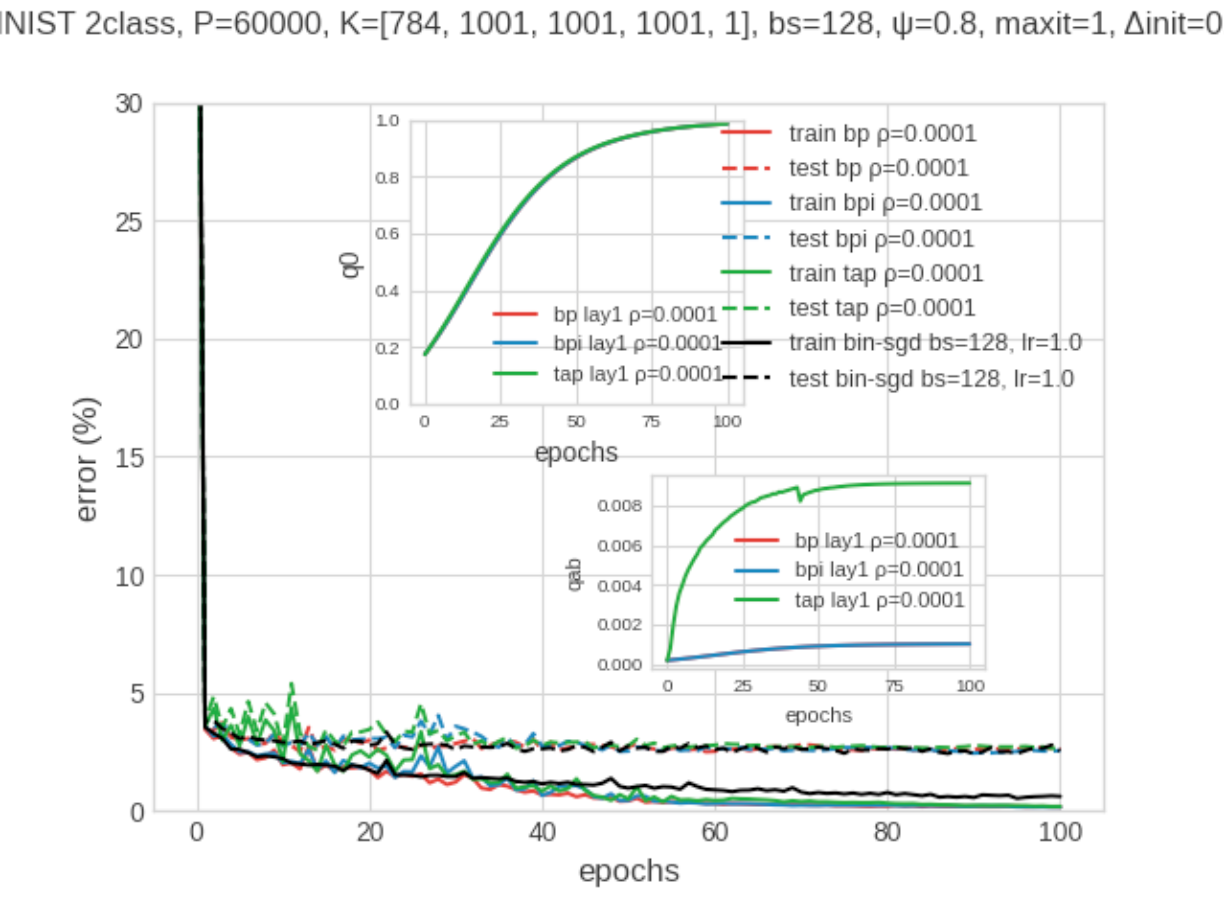
\includegraphics[scale=0.2]{figures/pasted/pasted34}

\caption{MLP with 3 hidden layers with 101/501/1001 hidden units each, batch-size=128
on the Fashion-MNIST dataset.}
\end{figure}
\par\end{center}

\subsection{Experiments on MNIST, FashionMNIST, CIFAR10 (10 classes)}
\begin{center}
\begin{figure}[H]
\includegraphics[scale=0.2]{figures/pasted_new/pasted25}\includegraphics[scale=0.2]{figures/pasted_new/pasted26}

\caption{MLP with 2 hidden layers with 101 hidden units each, batch-size=128
on the Fashion-MNIST dataset. (Left) argmax first version; (right)
argmax second version.}
\end{figure}
\par\end{center}

Cosa sto provando:
\begin{itemize}
\item 2 layer da 101; 2 layer da 1001 (per fittare di pi� il train) -> dovrei
fare anche una prova con 3 layer da 1001
\item batchsize 128 e 1
\item per SGD, lr=0.1,0.5,1
\item capire come scalano i tempi con la taglia degli hidden layer / la
profondit� -> sembra che non scalino bene con la taglia dell'hidden
layer, capire il motivo
\item effettivamente $\rho$ va fine-tunato sulla rete (cio� cambiando l'architettura
bisogna cambaire rho) -> per� prova a trovare il $\rho$ giusto sulla
rete da 1001-1001 e poi vedi se funziona pure su quella da 101-101
\end{itemize}

\subsection{Experiments on RFM}

Here we present results with the Random Features Model, concerning
in particular the permutation symmetry. In order to investigate the
role of the permutation symmetry we present results on the fully connected
committee machine (1 hidden layer network learning only the first
weight layer, with the weights of the second layer fixed to all ones).

The teacher in the latent space is a perceptron (check).
\begin{center}
\begin{figure}[H]
\begin{centering}
\includegraphics[scale=0.25]{figures/rfm_bp}
\par\end{centering}
\caption{Overlap varying $N$ in the RFM, fully connected committee machine
with various algorithms.}
\end{figure}
\par\end{center}
\end{document}
